

\section{JIT Design: The Big Picture}

In order for the \emph{JIT} tool to work with respect to the given requirements, we have come with certain necessary components that facilitate the workflow. As depicted in \autoref{fig:jit_module} under the \texttt{models}, we have the essential components responsible for representing and managing the models as Python objects before making them available to the \emph{NestKernel}. The \texttt{jit\_model} stores information about the chosen \emph{NESTML} model by storing its parameters and states and making it possible for the user to query on those attributes after creating the instances of the model. Secondly, we have the \texttt{model\_query} which is important for searching the model either in the \emph{nestml} files or in the created libraries. Depending on which format, the \texttt{model\_query} returns an instance of the \texttt{model\_handle}, which is responsible for making the model available to the \emph{NestKernel}. The  \texttt{model\_handle} knows if the model is coming from a \emph{nestml} file, and therefore can initiate the code generation process and install the model. On the other hand, if the model is coming from an already existing library, it will just install the model. The \texttt{model\_manager} is responsible for storing all created objects in the \emph{JIT} module, and it is the only way to communicate with the \emph{PyNEST} module. Additionally, the \texttt{model\_manager} manages the mapping of \emph{IDs} between the created models on the Python side and the real models coming from the \emph{NestKernel} with the help of the \texttt{model\_indexer}. Finally, under the \texttt{models} directory, we have the \texttt{node\_collection\_proxy} that mimics the behavior of the \texttt{nest.NodeCollection} in \emph{PyNEST} and it provides all functionalities like the \texttt{Setter/Getter} and \emph{Indexing/Slicing}. The need for such a class will be explained later on in this chapter. 


Under the \texttt{utils} directory, we have the needed components responsible for creating a \emph{lightweight} version of the \emph{nestml} models and controlling the code generation steps. The reason behind using a \emph{lightweight} version should also be clear in the following sections.

Furthermore, we have the \texttt{wrapper} directory containing the necessary logic for wrapping the \emph{PyNEST} targeted functions. In the \texttt{Wrapper.py} we have the \texttt{Wrapper} interface that contains the basic code needed for each wrapper to control the targeted functions and under \texttt{Wrappers.py} we have the derived concrete implementation of the \texttt{Wrapper}. Any further custom wrapping functionality should be added there, and it will be automatically registered. Details about how we can create a custom wrapper will be given later.

Finally, we have the \texttt{nest\_manager} which initiates the process of wrapping the \emph{PyNEST} module and calling the implemented wrappers for each target function. The \texttt{\_\_init\_\_} is obviously the starting point of the \emph{JIT} module that starts the \texttt{nest\_manager} and overrides the \texttt{import} function in Python in order to delegate any further imports from \emph{PyNEST} and add them to the \emph{JIT} module.



\begin{figure}[ht!]
\centering
\resizebox{\textwidth}{!}{
    \begin{tikzpicture}[
      level 1/.style={sibling distance=50mm},
      edge from parent/.style={->,draw},
      >=latex]
    
    % root of the the initial tree, level 1
    \node[root] {JIT}
    % The first level, as children of the initial tree
      child {node[level 2] (c1) {interfaces}}
      child {node[level 2] (c2) {models}}
      child {node[level 2] (c3) {utils}}
      child {node[level 2] (c4) {wrapper}}
      child {node[level 2] (c5) {nest\_manager.py}}
      child {node[level 2] (c6) {\_\_init\_\_.py}};
    
    % The second level, relatively positioned nodes
    \begin{scope}[every node/.style={level 3}]
    \node [below of = c1, xshift=25pt] (c11) {jit\_interface.py};
    
    \node [below of = c2, xshift=25pt] (c21) {jit\_model.py};
    \node [below of = c21] (c22) {model\_query.py};
    \node [below of = c22] (c23) {model\_indexer.py};
    \node [below of = c23] (c24) {model\_manager.py};
    \node [below of = c24] (c25) {model\_handle.py};
    \node [below of = c25] (c26) {node\_collection\_proxy.py};
    
    
    \node [below of = c3, xshift=25pt, fill=red!20] (c31) {templates};
    \node [below of = c31] (c32) {report.py};
    \node [below of = c32] (c33) {jit\_model\_parser.py};
    \node [below of = c33] (c34) {nest\_config.py};
    \node [below of = c34] (c35) {symbols.py};
    \node [below of = c35] (c36) {thread\_manager.py};
    \node [below of = c36] (c37) {utils.py};
    
    
    \node [below of = c4, xshift=25pt] (c41) {wrapper.py};
    \node [below of = c41] (c42) {wrappers.py};
    \node [below of = c42] (c43) {module\_wrapper.py};

    
    \end{scope}
    
    % lines from each level 1 node to every one of its "children"
    \foreach \value in {1}
      \draw[->] (c1.177) |- (c1\value.west);
    
    \foreach \value in {1,...,6}
      \draw[->] (c2.177) |- (c2\value.west);
    
    \foreach \value in {1,...,7}
      \draw[->] (c3.177) |- (c3\value.west);
      
      
    \foreach \value in {1,...,3}
      \draw[->] (c4.177) |- (c4\value.west);
    \end{tikzpicture}
    }
    \caption{The \emph{JIT} module components and subdirectories: The project is split into different subdirectories. The \emph{interfaces} folder contains the implemented folders. The \emph{models} folder contains the components responsible for managing the \emph{NESTML} models. The \emph{utils} directory is for providing tools that help with creating the models. The \emph{wraper} folder holds the implemented base \texttt{Wrapper} and its derived classes. }
    \label{fig:jit_module}

\end{figure}


In order to have a complete overview of what is happening in the back scene when running then \emph{JIT} tool, we have to explain the important steps in their correct order of execution. We start explaining the wrapping mechanism and how to implement our custom wrapper. Secondly, we explain how the creation of instances look like with \emph{JIT} tool enabled, and we discuss then how the \texttt{nest.Connect} function might be slightly modified and finally the role of the modified \texttt{nest.Simulate}. As the \texttt{NodeCollectionProxy} is part of the creation calls, we will introduce it in the same section of  the \texttt{nest.Create} wrapper.





\section{JIT Wrappers}

In this section, we introduce the \emph{Wrapper} interface responsible for intercepting the function calls in \emph{PyNEST}, and we discuss the derived classes inheriting from this interface allowing to control the workflow of the targeted functions in \emph{PyNEST}.

\subsection{The Wrapper Base Class}

The \emph{Wrapper} interface as depicted in \autoref{fig:wrapper_uml} shows the essential items that make \emph{JIT} module able to intercept and modify the calls to the \emph{high level API} in \emph{PyNESt}. Each \emph{Wrapper} instance has two boolean attributes. The first attribute specifies if we are wrapping a function or a method. The second is to ignore the function call and skip its execution. By default, the second attribute is set to \texttt{false}. As we have mentioned in the previous section, each \emph{Wrapper} object has three main functions to control the interception of the \emph{PyNEST} calls. the \texttt{before} function is mainly responsible for preprocessing the input values that are given to the \emph{PyNEST} function. Secondly, we have the \texttt{main}, which takes the modified parameters from the \texttt{before} function and executes the real \emph{PyNEST} wrapped function. Finally, we have the \texttt{after} function that takes the output of the \texttt{main} function and modifies it if necessary. In addition to those core functions, we have two important functions. The \texttt{get\_name} function that returns the name of the function that we want to wrap, and at last we have the \texttt{wraps\_one} that indicates if this \texttt{Wrapper} object is wrapping one or multiple functions. In the case if it is multiple functions, the \texttt{get\_name} function must return a list containing the names of these functions. One function left which brings all pieces together, the \texttt{\_\_wrapper} as it is responsible for calling the \texttt{before}, \texttt{main} and \texttt{after} functions.


\begin{figure}[ht!]
\centering
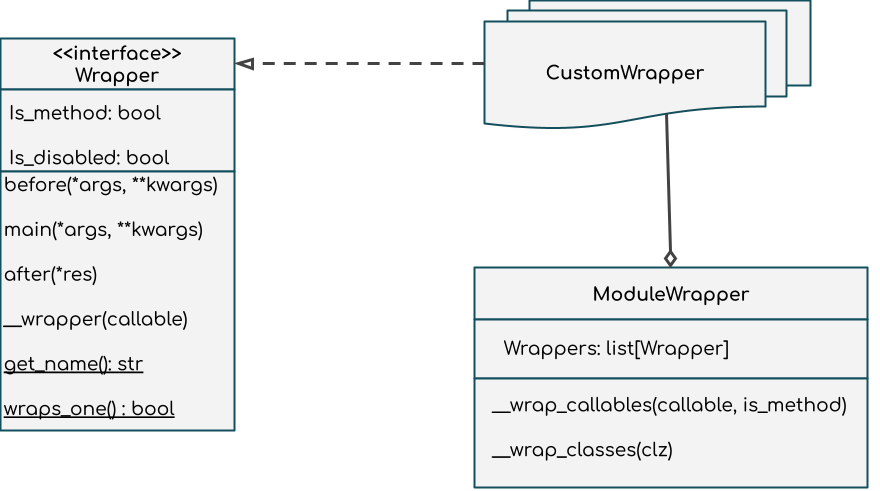
\includegraphics[width=\textwidth,height=\textheight,keepaspectratio]{src/pic/wrapper_uml.png}
\caption{The Wrapper interface: The Wrapper is the interface that controls the workflow of its derived classes. All \texttt{CustomWrapper} classes derived from the \texttt{Wrapper} may implement the \texttt{before, main} and \texttt{after} functions. The \texttt{\_\_wrapper} function is responsible for coordinating between the three main function and calling them in sequence. The static function \texttt{get\_name} specifies the target function or class in \emph{PyNEST}, and finally the other static function \texttt{wraps\_one} indicates how many \texttt{Wrapper} instances should be created. Additionally, we have the \texttt{ModuleWrapper} that is responsible for creating the \texttt{CustomWrapper} instances and matching them with their target functions in \emph{PyNEST}.}
\label{fig:wrapper_uml}
\end{figure}

The \texttt{ModuleWrapper} is responsible for matching the custom implemented wrappers with the targeted \emph{PyNEST} objects. It iterates overs all functions and classes and replaces them with their corresponding wrappers. finally, we have the \texttt{CustomWrappers} representing the derived classes from the \texttt{Wrapper} interface. Those derived classes can be seen in \autoref{fig:wrapper_derived}.

\subsection{The Wrapper Derived Classes}

The \emph{Wrapper} interface on its own does not do a lot for the \emph{JIT} project, and it requires having a concrete implementation for each function we want to control its workflow. Each derived class from the \emph{Wrapper} interface wraps either a \emph{function} or a \emph{class} in \emph{PyNEST}. As shown in \autoref{fig:wrapper_derived}, we depict the current implemented \emph{wrappers}. Most of these wrappers use a \texttt{helper} class that does all the required logic to make the \emph{JIT} approach work. In the following, we list the implemented wrappers and discuss their usage.

\begin{figure}[ht!]
\centering


\tikzset{every picture/.style={line width=0.75pt}} %set default line width to 0.75pt        

\begin{tikzpicture}[x=0.75pt,y=0.75pt,yscale=-1,xscale=1]
%uncomment if require: \path (0,519); %set diagram left start at 0, and has height of 519

%Rounded Rect [id:dp08332665529733485] 
\draw  [color={rgb, 255:red, 139; green, 87; blue, 42 }  ,draw opacity=1 ][line width=2.25]  (277,217) .. controls (277,212.58) and (280.58,209) .. (285,209) -- (395.8,209) .. controls (400.22,209) and (403.8,212.58) .. (403.8,217) -- (403.8,241) .. controls (403.8,245.42) and (400.22,249) .. (395.8,249) -- (285,249) .. controls (280.58,249) and (277,245.42) .. (277,241) -- cycle ;
%Rounded Rect [id:dp643201073355989] 
\draw  [color={rgb, 255:red, 139; green, 87; blue, 42 }  ,draw opacity=1 ][line width=2.25]  (1.8,427) .. controls (1.8,422.58) and (5.38,419) .. (9.8,419) -- (191.8,419) .. controls (196.22,419) and (199.8,422.58) .. (199.8,427) -- (199.8,451) .. controls (199.8,455.42) and (196.22,459) .. (191.8,459) -- (9.8,459) .. controls (5.38,459) and (1.8,455.42) .. (1.8,451) -- cycle ;
%Rounded Rect [id:dp9738213759503345] 
\draw  [color={rgb, 255:red, 139; green, 87; blue, 42 }  ,draw opacity=1 ][line width=2.25]  (2.8,262) .. controls (2.8,257.58) and (6.38,254) .. (10.8,254) -- (136.8,254) .. controls (141.22,254) and (144.8,257.58) .. (144.8,262) -- (144.8,286) .. controls (144.8,290.42) and (141.22,294) .. (136.8,294) -- (10.8,294) .. controls (6.38,294) and (2.8,290.42) .. (2.8,286) -- cycle ;
%Rounded Rect [id:dp39360724795655755] 
\draw  [color={rgb, 255:red, 139; green, 87; blue, 42 }  ,draw opacity=1 ][line width=2.25]  (503,349) .. controls (503,344.58) and (506.58,341) .. (511,341) -- (645.8,341) .. controls (650.22,341) and (653.8,344.58) .. (653.8,349) -- (653.8,373) .. controls (653.8,377.42) and (650.22,381) .. (645.8,381) -- (511,381) .. controls (506.58,381) and (503,377.42) .. (503,373) -- cycle ;
%Rounded Rect [id:dp2385264912044227] 
\draw  [color={rgb, 255:red, 139; green, 87; blue, 42 }  ,draw opacity=1 ][line width=2.25]  (255.8,480) .. controls (255.8,475.58) and (259.38,472) .. (263.8,472) -- (444.8,472) .. controls (449.22,472) and (452.8,475.58) .. (452.8,480) -- (452.8,504) .. controls (452.8,508.42) and (449.22,512) .. (444.8,512) -- (263.8,512) .. controls (259.38,512) and (255.8,508.42) .. (255.8,504) -- cycle ;
%Rounded Rect [id:dp04455155996593918] 
\draw  [color={rgb, 255:red, 139; green, 87; blue, 42 }  ,draw opacity=1 ][line width=2.25]  (153.8,33) .. controls (153.8,28.58) and (157.38,25) .. (161.8,25) -- (319.8,25) .. controls (324.22,25) and (327.8,28.58) .. (327.8,33) -- (327.8,57) .. controls (327.8,61.42) and (324.22,65) .. (319.8,65) -- (161.8,65) .. controls (157.38,65) and (153.8,61.42) .. (153.8,57) -- cycle ;
%Rounded Rect [id:dp5139694395821088] 
\draw  [color={rgb, 255:red, 139; green, 87; blue, 42 }  ,draw opacity=1 ][line width=2.25]  (5.8,100) .. controls (5.8,95.58) and (9.38,92) .. (13.8,92) -- (137.8,92) .. controls (142.22,92) and (145.8,95.58) .. (145.8,100) -- (145.8,124) .. controls (145.8,128.42) and (142.22,132) .. (137.8,132) -- (13.8,132) .. controls (9.38,132) and (5.8,128.42) .. (5.8,124) -- cycle ;
%Rounded Rect [id:dp796653880823329] 
\draw  [color={rgb, 255:red, 139; green, 87; blue, 42 }  ,draw opacity=1 ][line width=2.25]  (3.8,181) .. controls (3.8,176.58) and (7.38,173) .. (11.8,173) -- (129.8,173) .. controls (134.22,173) and (137.8,176.58) .. (137.8,181) -- (137.8,205) .. controls (137.8,209.42) and (134.22,213) .. (129.8,213) -- (11.8,213) .. controls (7.38,213) and (3.8,209.42) .. (3.8,205) -- cycle ;
%Rounded Rect [id:dp8115528255145159] 
\draw  [color={rgb, 255:red, 139; green, 87; blue, 42 }  ,draw opacity=1 ][line width=2.25]  (1.8,349) .. controls (1.8,344.58) and (5.38,341) .. (9.8,341) -- (159.8,341) .. controls (164.22,341) and (167.8,344.58) .. (167.8,349) -- (167.8,373) .. controls (167.8,377.42) and (164.22,381) .. (159.8,381) -- (9.8,381) .. controls (5.38,381) and (1.8,377.42) .. (1.8,373) -- cycle ;
%Rounded Rect [id:dp6414618614909982] 
\draw  [color={rgb, 255:red, 139; green, 87; blue, 42 }  ,draw opacity=1 ][line width=2.25]  (480.8,268) .. controls (480.8,263.58) and (484.38,260) .. (488.8,260) -- (645.8,260) .. controls (650.22,260) and (653.8,263.58) .. (653.8,268) -- (653.8,292) .. controls (653.8,296.42) and (650.22,300) .. (645.8,300) -- (488.8,300) .. controls (484.38,300) and (480.8,296.42) .. (480.8,292) -- cycle ;
%Rounded Rect [id:dp7381489249035267] 
\draw  [color={rgb, 255:red, 139; green, 87; blue, 42 }  ,draw opacity=1 ][line width=2.25]  (485.8,182) .. controls (485.8,177.58) and (489.38,174) .. (493.8,174) -- (648.8,174) .. controls (653.22,174) and (656.8,177.58) .. (656.8,182) -- (656.8,206) .. controls (656.8,210.42) and (653.22,214) .. (648.8,214) -- (493.8,214) .. controls (489.38,214) and (485.8,210.42) .. (485.8,206) -- cycle ;
%Rounded Rect [id:dp704574691668346] 
\draw  [color={rgb, 255:red, 139; green, 87; blue, 42 }  ,draw opacity=1 ][line width=2.25]  (476.8,102) .. controls (476.8,97.58) and (480.38,94) .. (484.8,94) -- (645.8,94) .. controls (650.22,94) and (653.8,97.58) .. (653.8,102) -- (653.8,126) .. controls (653.8,130.42) and (650.22,134) .. (645.8,134) -- (484.8,134) .. controls (480.38,134) and (476.8,130.42) .. (476.8,126) -- cycle ;
%Rounded Rect [id:dp33221553170106266] 
\draw  [color={rgb, 255:red, 139; green, 87; blue, 42 }  ,draw opacity=1 ][line width=2.25]  (381.8,32) .. controls (381.8,27.58) and (385.38,24) .. (389.8,24) -- (547.8,24) .. controls (552.22,24) and (555.8,27.58) .. (555.8,32) -- (555.8,56) .. controls (555.8,60.42) and (552.22,64) .. (547.8,64) -- (389.8,64) .. controls (385.38,64) and (381.8,60.42) .. (381.8,56) -- cycle ;
%Rounded Rect [id:dp11416390733512127] 
\draw  [color={rgb, 255:red, 139; green, 87; blue, 42 }  ,draw opacity=1 ][line width=2.25]  (499,425) .. controls (499,420.58) and (502.58,417) .. (507,417) -- (641.8,417) .. controls (646.22,417) and (649.8,420.58) .. (649.8,425) -- (649.8,449) .. controls (649.8,453.42) and (646.22,457) .. (641.8,457) -- (507,457) .. controls (502.58,457) and (499,453.42) .. (499,449) -- cycle ;
%Straight Lines [id:da7321475284754999] 
\draw [line width=1.5]  [dash pattern={on 1.69pt off 2.76pt}]  (144.8,113.6) -- (273.85,214.54) ;
\draw [shift={(277,217)}, rotate = 218.03] [fill={rgb, 255:red, 0; green, 0; blue, 0 }  ][line width=0.08]  [draw opacity=0] (11.61,-5.58) -- (0,0) -- (11.61,5.58) -- cycle    ;
%Straight Lines [id:da826027105738447] 
\draw [line width=1.5]  [dash pattern={on 1.69pt off 2.76pt}]  (141.8,191.6) -- (270.92,224.61) ;
\draw [shift={(274.8,225.6)}, rotate = 194.34] [fill={rgb, 255:red, 0; green, 0; blue, 0 }  ][line width=0.08]  [draw opacity=0] (11.61,-5.58) -- (0,0) -- (11.61,5.58) -- cycle    ;
%Straight Lines [id:da9419415019749295] 
\draw [line width=1.5]  [dash pattern={on 1.69pt off 2.76pt}]  (144.8,272.6) -- (269.98,233.78) ;
\draw [shift={(273.8,232.6)}, rotate = 162.77] [fill={rgb, 255:red, 0; green, 0; blue, 0 }  ][line width=0.08]  [draw opacity=0] (11.61,-5.58) -- (0,0) -- (11.61,5.58) -- cycle    ;
%Straight Lines [id:da2009447559522246] 
\draw [line width=1.5]  [dash pattern={on 1.69pt off 2.76pt}]  (169.8,364.6) -- (274.38,244.02) ;
\draw [shift={(277,241)}, rotate = 130.94] [fill={rgb, 255:red, 0; green, 0; blue, 0 }  ][line width=0.08]  [draw opacity=0] (11.61,-5.58) -- (0,0) -- (11.61,5.58) -- cycle    ;
%Curve Lines [id:da7600537285509692] 
\draw [line width=1.5]  [dash pattern={on 1.69pt off 2.76pt}]  (191.8,419) .. controls (249.32,402.03) and (261.22,290.39) .. (298.85,255.16) ;
\draw [shift={(301.8,252.6)}, rotate = 141.34] [fill={rgb, 255:red, 0; green, 0; blue, 0 }  ][line width=0.08]  [draw opacity=0] (11.61,-5.58) -- (0,0) -- (11.61,5.58) -- cycle    ;
%Straight Lines [id:da1297385545876295] 
\draw [line width=1.5]  [dash pattern={on 1.69pt off 2.76pt}]  (345.8,472.6) -- (341.09,255) ;
\draw [shift={(341,251)}, rotate = 88.76] [fill={rgb, 255:red, 0; green, 0; blue, 0 }  ][line width=0.08]  [draw opacity=0] (11.61,-5.58) -- (0,0) -- (11.61,5.58) -- cycle    ;
%Curve Lines [id:da8119155428391331] 
\draw [line width=1.5]  [dash pattern={on 1.69pt off 2.76pt}]  (492.8,433.6) .. controls (470.6,411.4) and (399.99,291.43) .. (381.59,258.8) ;
\draw [shift={(379.8,255.6)}, rotate = 60.95] [fill={rgb, 255:red, 0; green, 0; blue, 0 }  ][line width=0.08]  [draw opacity=0] (11.61,-5.58) -- (0,0) -- (11.61,5.58) -- cycle    ;
%Straight Lines [id:da43888705895379454] 
\draw [line width=1.5]  [dash pattern={on 1.69pt off 2.76pt}]  (500.8,367.6) -- (406.23,244.18) ;
\draw [shift={(403.8,241)}, rotate = 52.54] [fill={rgb, 255:red, 0; green, 0; blue, 0 }  ][line width=0.08]  [draw opacity=0] (11.61,-5.58) -- (0,0) -- (11.61,5.58) -- cycle    ;
%Straight Lines [id:da38095702214592175] 
\draw [line width=1.5]  [dash pattern={on 1.69pt off 2.76pt}]  (479.8,274.6) -- (411.17,230.75) ;
\draw [shift={(407.8,228.6)}, rotate = 32.57] [fill={rgb, 255:red, 0; green, 0; blue, 0 }  ][line width=0.08]  [draw opacity=0] (11.61,-5.58) -- (0,0) -- (11.61,5.58) -- cycle    ;
%Straight Lines [id:da685328333847449] 
\draw [line width=1.5]  [dash pattern={on 1.69pt off 2.76pt}]  (486.8,192.6) -- (407.64,215.87) ;
\draw [shift={(403.8,217)}, rotate = 343.62] [fill={rgb, 255:red, 0; green, 0; blue, 0 }  ][line width=0.08]  [draw opacity=0] (11.61,-5.58) -- (0,0) -- (11.61,5.58) -- cycle    ;
%Straight Lines [id:da09283567688019034] 
\draw [line width=1.5]  [dash pattern={on 1.69pt off 2.76pt}]  (473.8,119.6) -- (398.43,205.99) ;
\draw [shift={(395.8,209)}, rotate = 311.1] [fill={rgb, 255:red, 0; green, 0; blue, 0 }  ][line width=0.08]  [draw opacity=0] (11.61,-5.58) -- (0,0) -- (11.61,5.58) -- cycle    ;
%Curve Lines [id:da7212396930412046] 
\draw [line width=1.5]  [dash pattern={on 1.69pt off 2.76pt}]  (395.8,67.6) .. controls (378.34,64.69) and (399.46,164.34) .. (385.22,203.18) ;
\draw [shift={(383.8,206.6)}, rotate = 295.28] [fill={rgb, 255:red, 0; green, 0; blue, 0 }  ][line width=0.08]  [draw opacity=0] (11.61,-5.58) -- (0,0) -- (11.61,5.58) -- cycle    ;
%Straight Lines [id:da6247278152361431] 
\draw [line width=1.5]  [dash pattern={on 1.69pt off 2.76pt}]  (241.8,68.6) -- (337.46,201.35) ;
\draw [shift={(339.8,204.6)}, rotate = 234.22] [fill={rgb, 255:red, 0; green, 0; blue, 0 }  ][line width=0.08]  [draw opacity=0] (11.61,-5.58) -- (0,0) -- (11.61,5.58) -- cycle    ;

% Text Node
\draw (311,229) node [anchor=north west][inner sep=0.75pt]   [align=left] {{\fontfamily{pcr}\selectfont \textcolor[rgb]{0.55,0.34,0.16}{\textbf{Wrapper}}}};
% Text Node
\draw (8,430) node [anchor=north west][inner sep=0.75pt]   [align=left] {{\fontfamily{pcr}\selectfont \textbf{\textcolor[rgb]{0.55,0.34,0.16}{NodeCollectionWrapper}}}};
% Text Node
\draw (8,265) node [anchor=north west][inner sep=0.75pt]   [align=left] {{\fontfamily{pcr}\selectfont \textbf{\textcolor[rgb]{0.55,0.34,0.16}{DisableNestFunc}}}};
% Text Node
\draw (509,352) node [anchor=north west][inner sep=0.75pt]   [align=left] {\textbf{\textcolor[rgb]{0.55,0.34,0.16}{{\fontfamily{pcr}\selectfont GetStatusWrapper}}}};
% Text Node
\draw (265,482.5) node [anchor=north west][inner sep=0.75pt]   [align=left] {\textbf{\textcolor[rgb]{0.55,0.34,0.16}{\textbf{GetConnectionWrapper}}}};
% Text Node
\draw (175,38) node [anchor=north west][inner sep=0.75pt]   [align=left] {{\fontfamily{pcr}\selectfont \textcolor[rgb]{0.55,0.34,0.16}{\textbf{ConnectWrapper}}}};
% Text Node
\draw (20,103) node [anchor=north west][inner sep=0.75pt]   [align=left] {{\fontfamily{pcr}\selectfont \textbf{\textcolor[rgb]{0.55,0.34,0.16}{CreateWrapper}}}};
% Text Node
\draw (23,184) node [anchor=north west][inner sep=0.75pt]   [align=left] {\textbf{\textcolor[rgb]{0.55,0.34,0.16}{{\fontfamily{pcr}\selectfont ModelWrapper}}}};
% Text Node
\draw (11,352) node [anchor=north west][inner sep=0.75pt]   [align=left] {{\fontfamily{pcr}\selectfont \textbf{\textcolor[rgb]{0.55,0.34,0.16}{SimulationWrapper}}}};
% Text Node
\draw (492.3,273) node [anchor=north west][inner sep=0.75pt]   [align=left] {{\fontfamily{pcr}\selectfont \textbf{\textcolor[rgb]{0.55,0.34,0.16}{RestKernelWrapper}}}};
% Text Node
\draw (491,186) node [anchor=north west][inner sep=0.75pt]   [align=left] {\textbf{\textcolor[rgb]{0.55,0.34,0.16}{{\fontfamily{pcr}\selectfont GetDefaultsWrapper}}}};
% Text Node
\draw (487,106) node [anchor=north west][inner sep=0.75pt]   [align=left] {\textbf{\textcolor[rgb]{0.55,0.34,0.16}{{\fontfamily{pcr}\selectfont SetDefaultsWrapper}}}};
% Text Node
\draw (398,37) node [anchor=north west][inner sep=0.75pt]   [align=left] {{\fontfamily{pcr}\selectfont \textcolor[rgb]{0.55,0.34,0.16}{\textbf{CopyModelWrapper}}}};
% Text Node
\draw (505,430) node [anchor=north west][inner sep=0.75pt]   [align=left] {\textbf{\textcolor[rgb]{0.55,0.34,0.16}{{\fontfamily{pcr}\selectfont SetStatusWrapper}}}};
% Text Node
\draw (285,213) node [anchor=north west][inner sep=0.75pt]   [align=left] {{\fontfamily{pcr}\selectfont \textcolor[rgb]{0.55,0.34,0.16}{≪interface≫}}};


\end{tikzpicture}

\caption{The implemented \texttt{CustomWrapper} classes derived from the \texttt{Wrapper} interface.}
\label{fig:wrapper_derived}
\end{figure}




\begin{itemize}
   \item CreateWrapper: responsible for searching for the model in the \emph{file system} and in the \emph{NestKernel} built-in models and creating instances from it. \\
   
   \item ConnectWrapper:  responsible for making sure that we are always using the right model while calling the \texttt{nest.Connect} function. It may swap network elements depending on some conditions. \\
   
   \item CopyModelWrapper: shares the same functionality as the \texttt{CreateWrapper} for searching and installing the model in the \emph{NestKernel}. In addition, it creates a copy of the found model.
   
   \item SetStatusWrapper/GetStatusWrapper: set/get the status of the model's instances.\\
   
   
   \item SetDefaultWrapper/GetDefaultWrapper: set/get the default values of the model. Even if the model is not yet registered in the \emph{NestKernel}, the user can create  instances of the copied model.\\
   
   \item GetConnectionWrapper: returns the existing connections between source and target.
   
   \item ResetKernelWrapper: resets both the \emph{JIT} stored information about the models and  calls the \texttt{nest.ResetKerenel} function.\\
   
   \item NodeCollectionWrapper: returns an object containing the real object from the \emph{NestKernel} and the \emph{JIT} instances.\\
   
   \item ModelWrapper: returns all registered models from both the \emph{JIT} and \emph{NestKernel}.\\
   
   \item SimulationWrapper: makes sure that all \emph{JIT} instances are available in the \emph{NestKernel} to start the simulation.\\
   
   \item DisableNestFunc: skips the call of the \emph{PyNEST} function.
\end{itemize}   
   
   In the next step, we explain how to add a new wrapper in the \emph{JIT} module and explain the workflow behind the most important implemented wrappers. Mainly, the \texttt{CreateWrapper}, \texttt{ConnectWrapper} and \texttt{SimulateWrapper} are of interest, the others should follow the same logic.
   
   
\subsection{Adding a New Wrapper Class}

As shown in \ref{lst:custom_wrapper}, wrapping a new function or class in \emph{PyNEST} is very simple. We only need to add the new implementation to the \texttt{wrapper.py} Python file containing all implemented wrappers. At this point, there are no restrictions to how the \texttt{before-main-after} functions must be implemented. The implemented wrapper has the complete  control on how the target \emph{PyNEST} function should behave with respect to \emph{JIT} mechanism.


It is also important to know that the developer is not really required to provide an  implementation to the \texttt{before}, \texttt{main} and \texttt{after} functions. As for the default behavior of the \texttt{before} function will just return the input parameters unchanged, the \texttt{main} function calls the real \emph{PyNEST} function and finally the \texttt{after} function checks if \texttt{main} should return and just returns the same object unchanged, otherwise it does nothing.

Registering a custom \emph{Wrapper} is done automatically upon importing the \emph{JIT} module in the Python script. In The \texttt{wrappers.py} file, we have the \texttt{install\_wrappers} function shown in \autoref{lst:wrapper_reg} that is responsible for iterating over all the subclasses implementing the \texttt{Wrapper} interface and inserting them in a dictionary, having as \emph{key} the target function name and as \emph{value} the derived wrapper class. The \texttt{ModuleWrapper} imports then the dictionary and iterates over its keys, comparing them with \emph{PyNEST} functions and classes. Once a match is found, the \texttt{ModuleWrapper} creates an instance of the \texttt{CustomWrapper} and extends the \emph{JIT} module with a new function or class having the same name as the one coming from the \emph{PyNEST} module. The new inserted functions or classes in the \emph{JIT} module are either the original ones or an instance of the \texttt{CustomWrapper}.

\begin{figure}[ht!]
\centering
 \begin{lstlisting}[language=Python, label=lst:custom_wrapper, caption={CustomWrapper example}]
from jit.wrapper.wrapper import Wrapper

class CustomWrapper(Wrapper):

    def __init__(self, nest_func):
        super.__init__(nest_func, is_method=False, is_disabled=False)
        
    def __process_input(self, *args, **kwargs):
        # do something with the input
        return args, kwargs

    def __process_output(self, *res):
        # do something with the output
        return res
        
    def before(self, *args, **kwargs):
        return self.__process_input(args, kwargs)
    
    def main(self, *args, **kwargs):
        return self.nest_func(args, kwargs)
        
    def after(self, *res):
        return self.__process_output(res)
        
    @staticmethod
    def get_name():
        return "nest.{func_name}"
    
    @staticmethod
    def wraps_one():
        return True

\end{lstlisting}
    %\caption{CustomWrapper example}
    %\label{fig:custom_wrapper}
\end{figure}




\begin{figure}[ht!]
    \centering
    \begin{lstlisting}[language=Python, label=lst:wrapper_reg, caption={Registering Wrappers}]
def install_wrappers():
    sub_classes = Wrapper.__subclasses__()
    to_wrap = {}
    for sub_clz in sub_classes:
        if sub_clz.wrapps_one():
            to_wrap[sub_clz.get_name()] = sub_clz
        else:
            for name in sub_clz.get_name():
                to_wrap[name] = sub_clz
    return to_wrap
\end{lstlisting}
    %\caption{Registering Wrappers}
    %\label{fig:wrapper_reg}
\end{figure}





\section{PyNEST: The Creation Function}

Creating new models instances in \emph{PyNEST} is done by calling the create function \\\texttt{nest.Connect(model, n=1, params=None, positions=None)}. The first parameter should indicate the name of the model, the second is for telling \emph{PyNEST} how many instances we want to create, the third is for assigning new values for the attributes of those new instances and finally, the last parameter for indicating the spatial distribution of the created nodes. The return value of this function is a \texttt{NodeCollection} object, which is a compact and contiguous representation of the created nodes in the Python side. This \texttt{NodeCollection} objects stores only the \emph{first} and \emph{last} \emph{ids} of a continuous space of nodes \emph{ids}. Thus, if we create $n=10$ instances of any model and only select those odd or even positions, the \texttt{NodeCollection} object will have five blocks pointing to the individual odd/even positions. \autoref{fig:node_collection} shows an example how the \texttt{NodeCollection} may look like. At the start, we have only a single block containing the \texttt{first} and \texttt{last} \emph{ids} of the nodes. By splitting the created \texttt{NodeCollection} into even and odd \emph{ids}, we get two \texttt{NodeCollection} objects, each with five blocks. Each of these blocks points only to a single \emph{id}.


\begin{figure}[ht!]
\centering
\tikzset{every picture/.style={line width=0.75pt}} %set default line width to 0.75pt

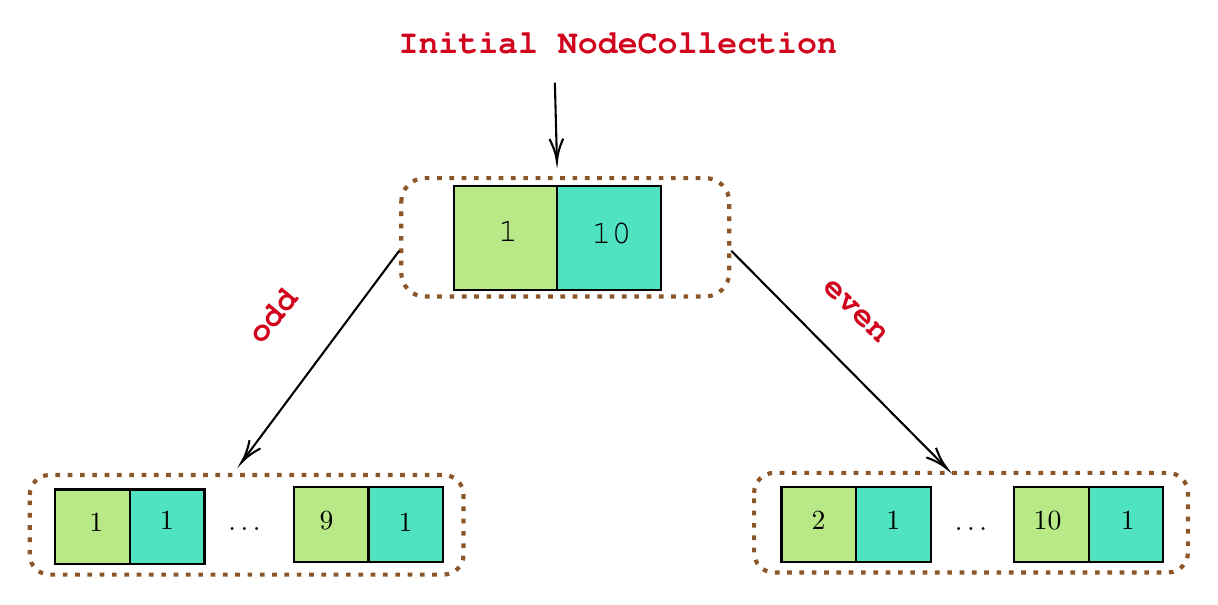
\begin{tikzpicture}[x=0.75pt,y=0.75pt,yscale=-1,xscale=1]
%uncomment if require: \path (0,420); %set diagram left start at 0, and has height of 420

%Shape: Square [id:dp14505338419362657] 
\draw  [fill={rgb, 255:red, 184; green, 233; blue, 134 }  ,fill opacity=1 ] (283,86) -- (333,86) -- (333,136) -- (283,136) -- cycle ;
%Shape: Square [id:dp5690214325454108] 
\draw  [fill={rgb, 255:red, 80; green, 227; blue, 194 }  ,fill opacity=1 ] (333,86) -- (383,86) -- (383,136) -- (333,136) -- cycle ;
%Rounded Rect [id:dp8563434876650051] 
\draw  [color={rgb, 255:red, 139; green, 87; blue, 42 }  ,draw opacity=1 ][dash pattern={on 1.69pt off 2.76pt}][line width=1.5]  (257.8,93.4) .. controls (257.8,87.1) and (262.9,82) .. (269.2,82) -- (404.4,82) .. controls (410.7,82) and (415.8,87.1) .. (415.8,93.4) -- (415.8,127.6) .. controls (415.8,133.9) and (410.7,139) .. (404.4,139) -- (269.2,139) .. controls (262.9,139) and (257.8,133.9) .. (257.8,127.6) -- cycle ;
%Shape: Square [id:dp7833262911739212] 
\draw  [fill={rgb, 255:red, 184; green, 233; blue, 134 }  ,fill opacity=1 ] (206,231) -- (242,231) -- (242,267) -- (206,267) -- cycle ;
%Shape: Square [id:dp9953924667288327] 
\draw  [fill={rgb, 255:red, 80; green, 227; blue, 194 }  ,fill opacity=1 ] (242,231) -- (278,231) -- (278,267) -- (242,267) -- cycle ;
%Shape: Square [id:dp6299533126736598] 
\draw  [fill={rgb, 255:red, 184; green, 233; blue, 134 }  ,fill opacity=1 ] (91,232) -- (127,232) -- (127,268) -- (91,268) -- cycle ;
%Shape: Square [id:dp19915315419671153] 
\draw  [fill={rgb, 255:red, 80; green, 227; blue, 194 }  ,fill opacity=1 ] (127,232) -- (163,232) -- (163,268) -- (127,268) -- cycle ;
%Shape: Square [id:dp5267204094552598] 
\draw  [fill={rgb, 255:red, 184; green, 233; blue, 134 }  ,fill opacity=1 ] (441,231) -- (477,231) -- (477,267) -- (441,267) -- cycle ;
%Shape: Square [id:dp7392648786591738] 
\draw  [fill={rgb, 255:red, 80; green, 227; blue, 194 }  ,fill opacity=1 ] (477,231) -- (513,231) -- (513,267) -- (477,267) -- cycle ;
%Shape: Square [id:dp2621212093475398] 
\draw  [fill={rgb, 255:red, 184; green, 233; blue, 134 }  ,fill opacity=1 ] (553,231) -- (589,231) -- (589,267) -- (553,267) -- cycle ;
%Shape: Square [id:dp328789805802878] 
\draw  [fill={rgb, 255:red, 80; green, 227; blue, 194 }  ,fill opacity=1 ] (589,231) -- (625,231) -- (625,267) -- (589,267) -- cycle ;
%Straight Lines [id:da7176298813855051] 
\draw    (331.8,36) -- (332.75,72) ;
\draw [shift={(332.8,74)}, rotate = 268.49] [color={rgb, 255:red, 0; green, 0; blue, 0 }  ][line width=0.75]    (10.93,-3.29) .. controls (6.95,-1.4) and (3.31,-0.3) .. (0,0) .. controls (3.31,0.3) and (6.95,1.4) .. (10.93,3.29)   ;
%Rounded Rect [id:dp5333242873793238] 
\draw  [color={rgb, 255:red, 139; green, 87; blue, 42 }  ,draw opacity=1 ][dash pattern={on 1.69pt off 2.76pt}][line width=1.5]  (78.8,234.6) .. controls (78.8,229.3) and (83.1,225) .. (88.4,225) -- (278.2,225) .. controls (283.5,225) and (287.8,229.3) .. (287.8,234.6) -- (287.8,263.4) .. controls (287.8,268.7) and (283.5,273) .. (278.2,273) -- (88.4,273) .. controls (83.1,273) and (78.8,268.7) .. (78.8,263.4) -- cycle ;
%Rounded Rect [id:dp9183238991512817] 
\draw  [color={rgb, 255:red, 139; green, 87; blue, 42 }  ,draw opacity=1 ][dash pattern={on 1.69pt off 2.76pt}][line width=1.5]  (427.8,233.6) .. controls (427.8,228.3) and (432.1,224) .. (437.4,224) -- (627.2,224) .. controls (632.5,224) and (636.8,228.3) .. (636.8,233.6) -- (636.8,262.4) .. controls (636.8,267.7) and (632.5,272) .. (627.2,272) -- (437.4,272) .. controls (432.1,272) and (427.8,267.7) .. (427.8,262.4) -- cycle ;
%Straight Lines [id:da22871011626744342] 
\draw    (256.8,117) -- (181.99,217.4) ;
\draw [shift={(180.8,219)}, rotate = 306.69] [color={rgb, 255:red, 0; green, 0; blue, 0 }  ][line width=0.75]    (10.93,-3.29) .. controls (6.95,-1.4) and (3.31,-0.3) .. (0,0) .. controls (3.31,0.3) and (6.95,1.4) .. (10.93,3.29)   ;
%Straight Lines [id:da2777097984312962] 
\draw    (416.8,117) -- (519.39,220.58) ;
\draw [shift={(520.8,222)}, rotate = 225.27] [color={rgb, 255:red, 0; green, 0; blue, 0 }  ][line width=0.75]    (10.93,-3.29) .. controls (6.95,-1.4) and (3.31,-0.3) .. (0,0) .. controls (3.31,0.3) and (6.95,1.4) .. (10.93,3.29)   ;
%Shape: Square [id:dp3719120065205612] 
\draw  [color={rgb, 255:red, 255; green, 255; blue, 255 }  ,draw opacity=1 ][fill={rgb, 255:red, 255; green, 255; blue, 255 }  ,fill opacity=1 ] (519.3,235) -- (545.3,235) -- (545.3,261) -- (519.3,261) -- cycle ;
%Shape: Square [id:dp3898179761369387] 
\draw  [color={rgb, 255:red, 255; green, 255; blue, 255 }  ,draw opacity=1 ][fill={rgb, 255:red, 255; green, 255; blue, 255 }  ,fill opacity=1 ] (170.3,236) -- (196.3,236) -- (196.3,262) -- (170.3,262) -- cycle ;

% Text Node
\draw (303,101) node [anchor=north west][inner sep=0.75pt]   [align=left] {{\fontfamily{pcr}\selectfont {\large 1}}};
% Text Node
\draw (348,102) node [anchor=north west][inner sep=0.75pt]   [align=left] {{\fontfamily{pcr}\selectfont {\large 10}}};
% Text Node
\draw (255,10) node [anchor=north west][inner sep=0.75pt]   [align=left] {{\fontfamily{pcr}\selectfont {\large \textcolor[rgb]{0.82,0.01,0.11}{\textbf{Initial NodeCollection}}}}};
% Text Node
\draw (106,242) node [anchor=north west][inner sep=0.75pt]   [align=left] {1};
% Text Node
\draw (140,241) node [anchor=north west][inner sep=0.75pt]   [align=left] {1};
% Text Node
\draw (454,241) node [anchor=north west][inner sep=0.75pt]   [align=left] {2};
% Text Node
\draw (490,241) node [anchor=north west][inner sep=0.75pt]   [align=left] {1};
% Text Node
\draw (603,241) node [anchor=north west][inner sep=0.75pt]   [align=left] {1};
% Text Node
\draw (217,241) node [anchor=north west][inner sep=0.75pt]   [align=left] {9};
% Text Node
\draw (255,242) node [anchor=north west][inner sep=0.75pt]   [align=left] {1};
% Text Node
\draw (561,241) node [anchor=north west][inner sep=0.75pt]   [align=left] {10};
% Text Node
\draw (180.34,156.35) node [anchor=north west][inner sep=0.75pt]  [rotate=-309.65] [align=left] {{\fontfamily{pcr}\selectfont {\large \textcolor[rgb]{0.82,0.01,0.11}{\textbf{odd}}}}};
% Text Node
\draw (465.4,128.02) node [anchor=north west][inner sep=0.75pt]  [rotate=-44.1] [align=left] {{\fontfamily{pcr}\selectfont {\large \textcolor[rgb]{0.82,0.01,0.11}{\textbf{even}}}}};
% Text Node
\draw (523,249) node [anchor=north west][inner sep=0.75pt]   [align=left] {\dots};
% Text Node
\draw (173,249) node [anchor=north west][inner sep=0.75pt]   [align=left] {\dots};


\end{tikzpicture}
\caption{Splitting a \texttt{NodeCollection} object: The initial \texttt{NodeCollection} instance has ten items, and instead of storing all the ten items, the \texttt{NodeCollection} stores only the first and the last \emph{ids} in the collection. Splitting the \texttt{NodeCollection} into even and odd \emph{ids}, we get two \texttt{NodeCollection} object, with each has five items. The separation of \emph{ids} in each split is due to non-contiguous space between them.}
\label{fig:node_collection}
\end{figure}


 In comparison to the initial block, the new blocks store only the \texttt{first} and the \texttt{size}. This happens because the blocks contain only a single item, but in the case of having blocks larger than one, they will have the same structure as the original block. It is important to know that the size of the \texttt{NodeCollection} object is computed by summing the size of each block. Thus, the size of the original \texttt{NodeCollection} instance is not one, but instead is $last - first + 1 = 10 - 1 + 1 =10$.
 
 As depicted in \autoref{fig:node_collection_agg}, aggregating \texttt{NodeCollection} objects results in having the original \texttt{NodeCollection} instance. Mainly, the logic behind the aggregation is to sort everything by \emph{id} at first, then aggregate the \emph{ids} by the model they belong to, merge them into blocks and finally split these blocks into contiguous spaces.\\
 
 \begin{figure}[ht!]

\tikzset{every picture/.style={line width=0.75pt}} %set default line width to 0.75pt        
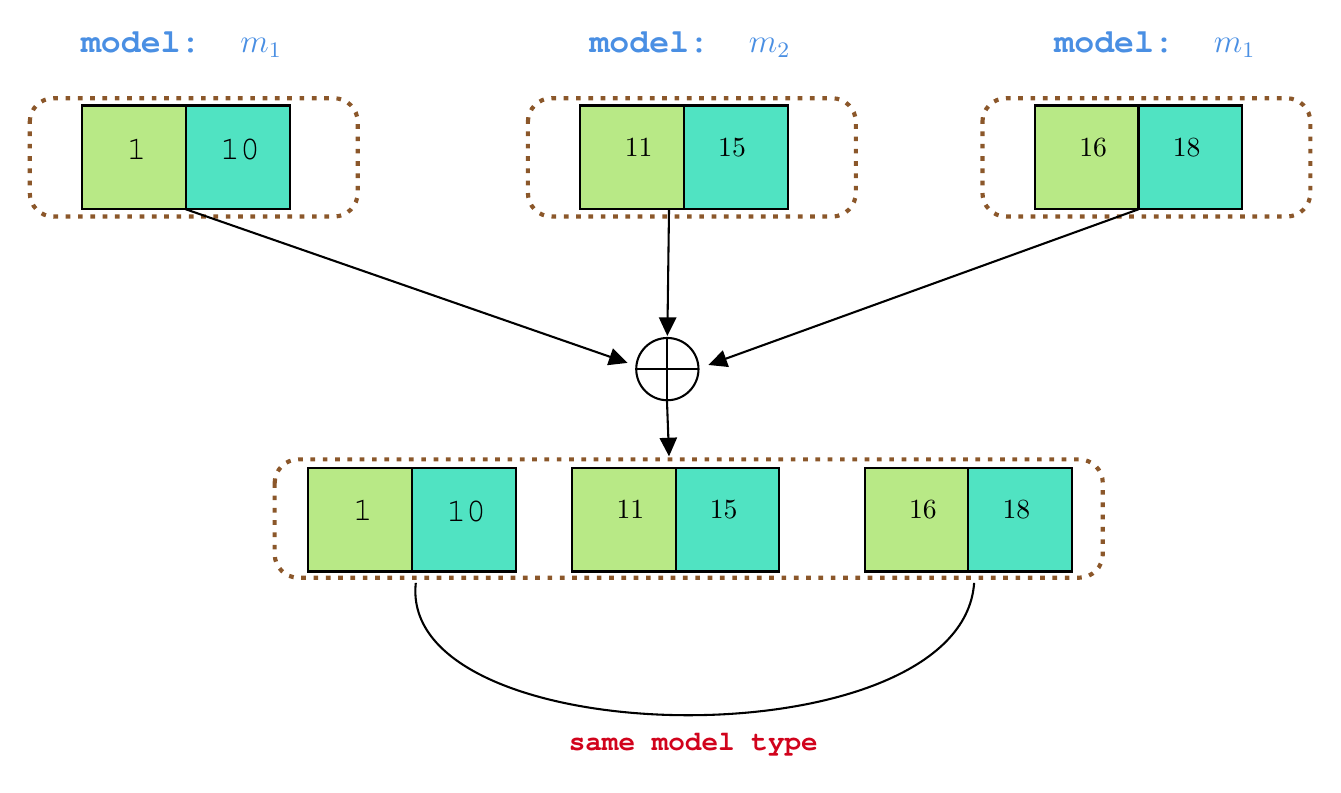
\begin{tikzpicture}[x=0.75pt,y=0.75pt,yscale=-1,xscale=1]
%uncomment if require: \path (0,420); %set diagram left start at 0, and has height of 420

%Shape: Square [id:dp847004206398758] 
\draw  [fill={rgb, 255:red, 184; green, 233; blue, 134 }  ,fill opacity=1 ] (41,42) -- (91,42) -- (91,92) -- (41,92) -- cycle ;
%Shape: Square [id:dp7413686977322151] 
\draw  [fill={rgb, 255:red, 80; green, 227; blue, 194 }  ,fill opacity=1 ] (91,42) -- (141,42) -- (141,92) -- (91,92) -- cycle ;
%Rounded Rect [id:dp9157715511667133] 
\draw  [color={rgb, 255:red, 139; green, 87; blue, 42 }  ,draw opacity=1 ][dash pattern={on 1.69pt off 2.76pt}][line width=1.5]  (15.8,49.9) .. controls (15.8,43.6) and (20.9,38.5) .. (27.2,38.5) -- (162.4,38.5) .. controls (168.7,38.5) and (173.8,43.6) .. (173.8,49.9) -- (173.8,84.1) .. controls (173.8,90.4) and (168.7,95.5) .. (162.4,95.5) -- (27.2,95.5) .. controls (20.9,95.5) and (15.8,90.4) .. (15.8,84.1) -- cycle ;
%Shape: Square [id:dp7126705161517422] 
\draw  [fill={rgb, 255:red, 184; green, 233; blue, 134 }  ,fill opacity=1 ] (281,42) -- (331,42) -- (331,92) -- (281,92) -- cycle ;
%Shape: Square [id:dp6046869167773221] 
\draw  [fill={rgb, 255:red, 80; green, 227; blue, 194 }  ,fill opacity=1 ] (331,42) -- (381,42) -- (381,92) -- (331,92) -- cycle ;
%Rounded Rect [id:dp7623925132527456] 
\draw  [color={rgb, 255:red, 139; green, 87; blue, 42 }  ,draw opacity=1 ][dash pattern={on 1.69pt off 2.76pt}][line width=1.5]  (255.8,49.9) .. controls (255.8,43.6) and (260.9,38.5) .. (267.2,38.5) -- (402.4,38.5) .. controls (408.7,38.5) and (413.8,43.6) .. (413.8,49.9) -- (413.8,84.1) .. controls (413.8,90.4) and (408.7,95.5) .. (402.4,95.5) -- (267.2,95.5) .. controls (260.9,95.5) and (255.8,90.4) .. (255.8,84.1) -- cycle ;
%Shape: Square [id:dp23969321871465432] 
\draw  [fill={rgb, 255:red, 184; green, 233; blue, 134 }  ,fill opacity=1 ] (500,42) -- (550,42) -- (550,92) -- (500,92) -- cycle ;
%Shape: Square [id:dp5973854844810629] 
\draw  [fill={rgb, 255:red, 80; green, 227; blue, 194 }  ,fill opacity=1 ] (550,42) -- (600,42) -- (600,92) -- (550,92) -- cycle ;
%Rounded Rect [id:dp4358433234191832] 
\draw  [color={rgb, 255:red, 139; green, 87; blue, 42 }  ,draw opacity=1 ][dash pattern={on 1.69pt off 2.76pt}][line width=1.5]  (474.8,49.9) .. controls (474.8,43.6) and (479.9,38.5) .. (486.2,38.5) -- (621.4,38.5) .. controls (627.7,38.5) and (632.8,43.6) .. (632.8,49.9) -- (632.8,84.1) .. controls (632.8,90.4) and (627.7,95.5) .. (621.4,95.5) -- (486.2,95.5) .. controls (479.9,95.5) and (474.8,90.4) .. (474.8,84.1) -- cycle ;
%Shape: Square [id:dp6913149663475422] 
\draw  [fill={rgb, 255:red, 184; green, 233; blue, 134 }  ,fill opacity=1 ] (150,216.5) -- (200,216.5) -- (200,266.5) -- (150,266.5) -- cycle ;
%Shape: Square [id:dp9939502562728053] 
\draw  [fill={rgb, 255:red, 80; green, 227; blue, 194 }  ,fill opacity=1 ] (200,216.5) -- (250,216.5) -- (250,266.5) -- (200,266.5) -- cycle ;
%Rounded Rect [id:dp2894941589728419] 
\draw  [color={rgb, 255:red, 139; green, 87; blue, 42 }  ,draw opacity=1 ][dash pattern={on 1.69pt off 2.76pt}][line width=1.5]  (133.8,223.9) .. controls (133.8,217.6) and (138.9,212.5) .. (145.2,212.5) -- (521.4,212.5) .. controls (527.7,212.5) and (532.8,217.6) .. (532.8,223.9) -- (532.8,258.1) .. controls (532.8,264.4) and (527.7,269.5) .. (521.4,269.5) -- (145.2,269.5) .. controls (138.9,269.5) and (133.8,264.4) .. (133.8,258.1) -- cycle ;
%Shape: Square [id:dp6685853677708664] 
\draw  [fill={rgb, 255:red, 184; green, 233; blue, 134 }  ,fill opacity=1 ] (277,216.5) -- (327,216.5) -- (327,266.5) -- (277,266.5) -- cycle ;
%Shape: Square [id:dp4147175960535616] 
\draw  [fill={rgb, 255:red, 80; green, 227; blue, 194 }  ,fill opacity=1 ] (327,216.5) -- (377,216.5) -- (377,266.5) -- (327,266.5) -- cycle ;
%Shape: Square [id:dp512011435333084] 
\draw  [fill={rgb, 255:red, 184; green, 233; blue, 134 }  ,fill opacity=1 ] (418,216.5) -- (468,216.5) -- (468,266.5) -- (418,266.5) -- cycle ;
%Shape: Square [id:dp4778634283532628] 
\draw  [fill={rgb, 255:red, 80; green, 227; blue, 194 }  ,fill opacity=1 ] (468,216.5) -- (518,216.5) -- (518,266.5) -- (468,266.5) -- cycle ;
%Straight Lines [id:da2340156449095352] 
\draw [line width=0.75]    (91,92) -- (300.97,165.01) ;
\draw [shift={(303.8,166)}, rotate = 199.17] [fill={rgb, 255:red, 0; green, 0; blue, 0 }  ][line width=0.08]  [draw opacity=0] (8.93,-4.29) -- (0,0) -- (8.93,4.29) -- cycle    ;
%Straight Lines [id:da9639225095005677] 
\draw    (323.8,92) -- (323.04,150) ;
\draw [shift={(323,153)}, rotate = 270.75] [fill={rgb, 255:red, 0; green, 0; blue, 0 }  ][line width=0.08]  [draw opacity=0] (8.93,-4.29) -- (0,0) -- (8.93,4.29) -- cycle    ;
%Straight Lines [id:da2987801737891538] 
\draw    (550,92) -- (345.62,165.98) ;
\draw [shift={(342.8,167)}, rotate = 340.1] [fill={rgb, 255:red, 0; green, 0; blue, 0 }  ][line width=0.08]  [draw opacity=0] (8.93,-4.29) -- (0,0) -- (8.93,4.29) -- cycle    ;
\draw   (308,169) .. controls (308,160.72) and (314.72,154) .. (323,154) .. controls (331.28,154) and (338,160.72) .. (338,169) .. controls (338,177.28) and (331.28,184) .. (323,184) .. controls (314.72,184) and (308,177.28) .. (308,169) -- cycle ; \draw   (308,169) -- (338,169) ; \draw   (323,154) -- (323,184) ;
%Straight Lines [id:da9446189905883726] 
\draw    (322.8,184) -- (323.69,208) ;
\draw [shift={(323.8,211)}, rotate = 267.88] [fill={rgb, 255:red, 0; green, 0; blue, 0 }  ][line width=0.08]  [draw opacity=0] (8.93,-4.29) -- (0,0) -- (8.93,4.29) -- cycle    ;
%Shape: Boxed Bezier Curve [id:dp5511245545993457] 
\draw    (201.8,272) .. controls (192.8,355) and (464.8,359) .. (470.8,272) ;

% Text Node
\draw (61,56.5) node [anchor=north west][inner sep=0.75pt]   [align=left] {{\fontfamily{pcr}\selectfont {\large 1}}};
% Text Node
\draw (106,56.5) node [anchor=north west][inner sep=0.75pt]   [align=left] {{\fontfamily{pcr}\selectfont {\large 10}}};
% Text Node
\draw (301,56.5) node [anchor=north west][inner sep=0.75pt]   [align=left] {11};
% Text Node
\draw (346,56.5) node [anchor=north west][inner sep=0.75pt]   [align=left] {15};
% Text Node
\draw (520,56.5) node [anchor=north west][inner sep=0.75pt]   [align=left] {16};
% Text Node
\draw (565,56.5) node [anchor=north west][inner sep=0.75pt]   [align=left] {18};
% Text Node
\draw (284,5) node [anchor=north west][inner sep=0.75pt]   [align=left] {{\fontfamily{pcr}\selectfont {\large \textbf{\textcolor[rgb]{0.29,0.56,0.89}{model: $m_2$}}}}};
% Text Node
\draw (508,5) node [anchor=north west][inner sep=0.75pt]   [align=left] {{\fontfamily{pcr}\selectfont {\large \textcolor[rgb]{0.29,0.56,0.89}{\textbf{model: $m_1$}}}}};
% Text Node
\draw (39,5) node [anchor=north west][inner sep=0.75pt]   [align=left] {{\fontfamily{pcr}\selectfont {\large \textcolor[rgb]{0.29,0.56,0.89}{\textbf{model: $m_1$}}}}};
% Text Node
\draw (170,230.5) node [anchor=north west][inner sep=0.75pt]   [align=left] {{\fontfamily{pcr}\selectfont {\large 1}}};
% Text Node
\draw (215,231) node [anchor=north west][inner sep=0.75pt]   [align=left] {{\fontfamily{pcr}\selectfont {\large 10}}};
% Text Node
\draw (297,231) node [anchor=north west][inner sep=0.75pt]   [align=left] {11};
% Text Node
\draw (342,231) node [anchor=north west][inner sep=0.75pt]   [align=left] {15};
% Text Node
\draw (438,231) node [anchor=north west][inner sep=0.75pt]   [align=left] {16};
% Text Node
\draw (483,231) node [anchor=north west][inner sep=0.75pt]   [align=left] {18};
% Text Node
\draw (274,343) node [anchor=north west][inner sep=0.75pt]   [align=left] {\textcolor[rgb]{0.82,0.01,0.11}{{\fontfamily{pcr}\selectfont \textbf{same model type}}}};


\end{tikzpicture}
\caption{Aggregation of \texttt{NodeCollection} objects: We start with two models $m_1$ and $m_2$. The first model $m_1$ has two \texttt{NodeCollection} objects pointing to it. The first collection has ten items with \emph{ids} between 1 and 10, and the second collection has only three items with \emph{ids} between 16 and 18. The second model $m_2$ has only one collection with five elements with \emph{ids} between 11 and 15. The aggregation of the three \texttt{NodeCollection} instances results in a once \texttt{NodeCollection} object that handles the items as a single list, but also it keeps the separation between the models and their \emph{ids}. }
\label{fig:node_collection_agg}
\end{figure}

A pre-condition for the \texttt{nest.Create} function to work and to return an instance of the \texttt{NodeCollection} object is to have the \emph{model} registered in the \emph{NestKenel} (see \autoref{chap:funds}). The desired \emph{model} is either already installed as a \emph{built-in model} in the \emph{NestKernel} or it must be manually installed by first running the code generation pipeline and calling the \texttt{nest.Install} method. These steps must be manually and repeatedly done in any simulation script trying to use an \emph{external model} that is not already available in the \emph{NestKernel}. To automate this process, the \texttt{nest.Create} function must know in advance where to find the given model, register it and make it available for use without having the user explicitly calling the code generator and the \texttt{nest.Install} function. For these purpose, we have the \texttt{CreateWrapper}, which exactly solves the problem by preparing everything automatically before calling the \texttt{nest.Create} function. In the following subsection, we will discuss the work flow of the \texttt{CreateWrapper} and discuss the important implemented logic to make it work correctly.

%\subsection{The CreateWrapper}

Recall in \autoref{chap:funds}, precisely in \autoref{fig:pynestml_workflow}, we have split the code generation process into three steps. The Parsing and validation, the transformation and finally the code generation and building the extension module. The simulation script can be split into three phases. At first, we have to create the nodes and, depending on the simulation scenario, some nodes might need to have some random configurations and thus the user might want to inspect the drawn values and apply some pre-analysis for the current state of these nodes. Secondly, once the nodes are ready, we proceed to the next step and connect the nodes and create the network. Similar to the nodes, the network can be a \emph{random network}, where nodes are connected with probability $p$. Once the network is set and the random parameters are drawn, the user can inspect the topology of the network. The last step in the simulation script is to simply run the \texttt{nest.Simulate(t)} function and wait for the simulation to finish, and afterward the user can then analyze the behavior of the network and check the final reached state of the nodes. It is important to know that the configuration of the nodes and the of the network are two separate things, and they do not influence each other. The \texttt{CreateWrapper} makes use of this separation by splitting the code generation pipeline into two steps. The first step uses only the parsing and the transformation steps, whereas the code generation and building the extension module is executed in the background and the \texttt{nest.Create} function will not wait for the complete code generation pipeline to finish.

The main tasks for the \texttt{CreateWrapper} are to firstly search for the specified model in the \emph{built-in} models, in the existing folders of the built libraries and finally in the folders containing the \texttt{.nestml} files. For the first case that the model is a \emph{built-in} model, the \texttt{CreateWrapper} simply calls \texttt{nest.Create} with the provided parameters. If the model already exists in one of the external libraries, then the wrapper calls the \texttt{nest.Install} function to register the model and then calls the \texttt{nest.Create}. In the worst scenario case, the model's library does not really exist, and therefore the code generation pipeline must be executed. Recall again that we first reach the transformation phase, then we generate a \emph{lightweight} version of the model by extracting its parameters and states and making them  directly available after the create call. The code generation and building  of the library is done then in a background process. Only the \texttt{nest.Connect} and \texttt{nest.Simulate} functions can check the status of the running background process and on success the complete model will be registered, and it will be complete available.


In order for the \texttt{CreateWrapper} to hide all these steps for making the model available after the create call, we need to have a class similar to the \texttt{NodeCollection} that works on the \emph{lightweight-partial} version of the model. The name of this class is called the \texttt{NodeCollectionProxy}, and it will be explained later in this section. Along with this new class, the \texttt{CreateWrapper} uses a help class called the \texttt{CreateHelper} that takes responsibility for searching for the model and making it either completely or partially ready to query and to modify. All these components will be discussed in the following subsections.

\subsection{The CreateWrapper}

Due to the simple \texttt{Wrapper} interface, the \texttt{CreateWrapper} as depicted in \autoref{lst:create_wrapper} uses only the \texttt{CreateHelper} that encapsulates the logic behind the \texttt{nest.Create} function. The \texttt{CreateHelper} has a \texttt{create} function that has the same signature as the  \texttt{nest.Create}, but instead of returning a \texttt{NodeCollection} object, it returns a \texttt{NodeCollectionProxy} object. All of those steps are done in the \texttt{before} function, and the \texttt{NodeCollectionProxy} object is stored as a member object of the \texttt{CreateWrapper} class. As the \texttt{main} function is completely ignored in this context, the \texttt{before} function returns just an empty tuple and an empty dictionary. Finally, the \texttt{after} function returns the stored \texttt{NodeCollectionProxy} object, and it does nothing else.

\begin{figure}[ht!]
    \centering
    \begin{lstlisting}[language=Python, label=lst:create_wrapper, caption={The \texttt{CreateWrapper}}]
from jit.helpers.create_helper import CreateHelper
from jit.wrapper.wrapper import Wrapper

class CreateWrapper(Wrapper):

    def __init__(self, func):
        super().__init__(func, is_method=False, is_disabled=False)
        self.nodeCollectionProxy = None
        
    def before(self, model_name, n=1, params=None, positions=None):
        createHelper = CreateHelper()
        self.nodeCollectionProxy = createHelper.Create(
                                   model_name, n, params, positions)
        return (), {}
    
    def main(self, *args, **kwargs):
        pass
    
    def after(self, *res):
        return self.nodeCollectionProxy
    
    @staticmethod
    def get_name():
        return "nest.Create"
\end{lstlisting}
    %\caption{}
    %\label{fig:create_wrapper}
\end{figure}




\subsection{The CreateHelper}

The \texttt{CreateHelper} is the essential component for controlling the workflow of the \texttt{nest.Create} function. In order to understand what is really happening in each of the functions in the \autoref{lst:create_helper}, we need to understand the role of each of the import lines. The first line \emph{imports} the \texttt{ModelQuery} which responsible for finding the model and returning its \emph{handle} that knows if the model is coming from a \emph{nestml} file or from a library. The second line is for importing the \texttt{NodeCollectionProxy} that mimics the functionality of the \texttt{NodeCollection}. The \texttt{ModelManager} in the third line holds the \texttt{nest} module, with which the \texttt{CreateHelper} can call the \texttt{nest.Create} function. The fourth line contains three important elements for the \emph{JIT} approach to work. The \texttt{JitModel} stores information about the model, like the states and parameters and their default values. The \texttt{JitNode} is a compact contiguous representation for the created instances. It stores the name of the model, the \emph{first} and the \emph{last ids} of the instances. Finally, we have the \texttt{JitNodeCollection} which is a list of \texttt{JitNode}s. In Short, if we have a tree like, the \texttt{JitNodeCollection} will be the root, the \texttt{JitNode}s are the direct children of the root and the \texttt{JitModel}s are the leaves. The last import line is the \texttt{JitThread} which responsible for running the code generation and the building of the library in the background.
\begin{figure}[ht!]
    \centering
    \begin{lstlisting}[language=Python, label=lst:create_helper, caption={The CreateHelper}]
from jit.models.model_query import ModelQuery
from jit.models.node_collection_proxy import NodeCollectionProxy
from jit.models.model_manager import ModelManager
from jit.models.jit_model import JitModel, JitNode, JitNodeCollection
from jit.utils.thread_manager import JitThread


class CreateHelper:
    def __init__(self):
        # create an empty NodeCollectionProxy instance
        self.nodeCollectionProxy = NodeCollectionProxy()
    def Create(self, model_name, n=1, params=None, positions=None):
        # handle different cases
        
    def handle_built_in(self, model_name, n=1, params=None, positions=None):
        pass
        
    def handle_external_lib(self, model_name, n=1, params=None, positions=None):
        pass
    
    def handle_nestml(self, model_name, n=1, params=None, positions=None): 
        pass
        
    def handle_jit_model(self, model_name, n=1, params=None, positions=None):
        pass
    
\end{lstlisting}
    %\caption{The \texttt{CreateHelper}}
    %\label{fig:create_helper}
\end{figure}

The explanation of the \texttt{Create} function will be left as the last function to discuss. We start with the \texttt{handle\_built\_in} method. It is the simplest case, where we just call the real create function from the \emph{PyNEST} module, and then we store the \texttt{NodeCollection} returned object in the \texttt{NodeCollectionProxy}. An important part of the \texttt{CreateHelper} is to keep the order of \emph{ids} consistent. With the help of the \texttt{ModelManager}, we can query the last assigned \emph{id} and update it with the size of the \texttt{NodeCollection}. Finaly, we store the \texttt{NodeCollectionProxy} in an array of nodeCollectionProxies in the \texttt{ModelManager}.

The task of the \texttt{handle\_external\_lib} can be split into two parts. The second part is exactly like the \texttt{handle\_built\_in} function. The first part takes care of installing the library.

Now to the most important part, the \texttt{handle\_nestml} function that is responsible for making the \emph{nestml} model available in the simulation. The process starts by asking the \emph{handle} to start processing the model by doing the first two steps in the code generation (i.e., Parsing and Transformation). The \texttt{ModelHanlde.get\_models} function is then called to iterate over the \texttt{ASTNeuron} and \texttt{ASTSynapse} objects and create the \emph{lightweight} version of the model that has only the \emph{state} and \emph{parameter} blocks of the model. Once the \emph{lightweight} version is returned from the  \texttt{ModelHanlde.get\_models} function, the \texttt{handle\_nestml} checks then if the provided attributes names and types are correct or not and then gives the control to the \texttt{handle\_jit\_model}, where the \texttt{JitNodeCollection} object is created and stored in the \texttt{NodeCollectionProxy}. After that, the  \texttt{handle\_nestml} resumes and initiates the thread to work in the background to generate the library code and build it. The  \texttt{handle\_jit\_model} can also be executed separately from the  \texttt{handle\_nestml}, as it may happen that the simulation script may request the same model twice before it becomes available, and therefore we do not really have to execute the search for the model and initiate the code generation pipeline, but instead we update the \texttt{JitModel} instance by extending its internal structure to store information about the new desired instances.


Finally, we have the \texttt{Create} function that calls all the above described methods. It first checks if the \texttt{ModelManager} has already seen the \texttt{JitModel} with the given name. If it is the case, then the \texttt{handle\_jit\_model} method will be called, otherwise we check if the model is in the \emph{built\_in} models and then call the  \texttt{handle\_built\_in}. If the model name is neither registered in the \texttt{JitModel}s nor in the \emph{built\_in} models, we check the \texttt{ModelHandle} instance if the model is coming from a library or a \emph{nestml} file. For the first case we call the  \texttt{handle\_external\_lib} and for the second one we call the  \texttt{handle\_nestml} function. Independent of what was executed, the \texttt{Create} function returns a \texttt{NodeCollectionProxy} object that can hold both a \texttt{NodeCollection} and a \texttt{JitNodeCollection}. 

\subsection{The NodeCollectionProxy}

\begin{figure}[ht!]

\tikzset{every picture/.style={line width=0.75pt}} %set default line width to 0.75pt        

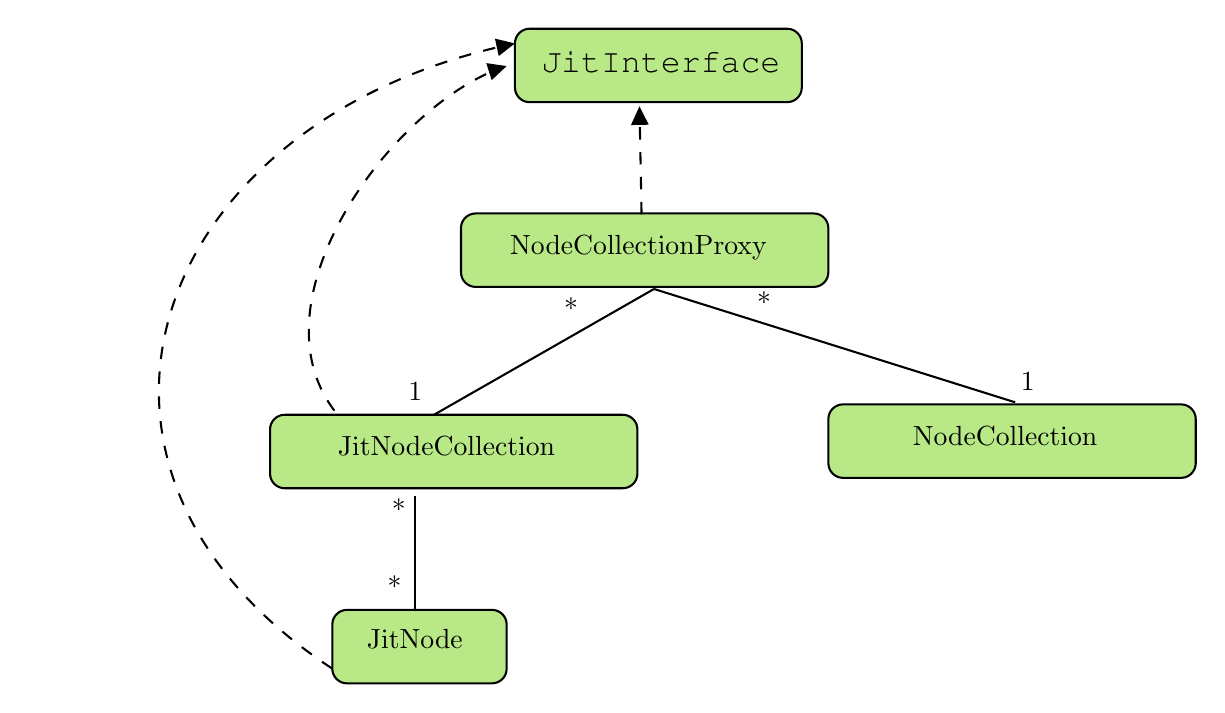
\begin{tikzpicture}[x=0.75pt,y=0.75pt,yscale=-1,xscale=1]
%uncomment if require: \path (0,539); %set diagram left start at 0, and has height of 539

%Rounded Rect [id:dp9242718804018157] 
\draw  [fill={rgb, 255:red, 184; green, 233; blue, 134 }  ,fill opacity=1 ] (258.8,21.08) .. controls (258.8,17.17) and (261.97,14) .. (265.88,14) -- (389.92,14) .. controls (393.83,14) and (397,17.17) .. (397,21.08) -- (397,42.32) .. controls (397,46.23) and (393.83,49.4) .. (389.92,49.4) -- (265.88,49.4) .. controls (261.97,49.4) and (258.8,46.23) .. (258.8,42.32) -- cycle ;
%Rounded Rect [id:dp20300555302885148] 
\draw  [fill={rgb, 255:red, 184; green, 233; blue, 134 }  ,fill opacity=1 ] (232.8,110.08) .. controls (232.8,106.17) and (235.97,103) .. (239.88,103) -- (402.72,103) .. controls (406.63,103) and (409.8,106.17) .. (409.8,110.08) -- (409.8,131.32) .. controls (409.8,135.23) and (406.63,138.4) .. (402.72,138.4) -- (239.88,138.4) .. controls (235.97,138.4) and (232.8,135.23) .. (232.8,131.32) -- cycle ;
%Rounded Rect [id:dp30259215827088815] 
\draw  [fill={rgb, 255:red, 184; green, 233; blue, 134 }  ,fill opacity=1 ] (140.8,207.08) .. controls (140.8,203.17) and (143.97,200) .. (147.88,200) -- (310.72,200) .. controls (314.63,200) and (317.8,203.17) .. (317.8,207.08) -- (317.8,228.32) .. controls (317.8,232.23) and (314.63,235.4) .. (310.72,235.4) -- (147.88,235.4) .. controls (143.97,235.4) and (140.8,232.23) .. (140.8,228.32) -- cycle ;
%Rounded Rect [id:dp43198649276984225] 
\draw  [fill={rgb, 255:red, 184; green, 233; blue, 134 }  ,fill opacity=1 ] (409.8,202.08) .. controls (409.8,198.17) and (412.97,195) .. (416.88,195) -- (579.72,195) .. controls (583.63,195) and (586.8,198.17) .. (586.8,202.08) -- (586.8,223.32) .. controls (586.8,227.23) and (583.63,230.4) .. (579.72,230.4) -- (416.88,230.4) .. controls (412.97,230.4) and (409.8,227.23) .. (409.8,223.32) -- cycle ;
%Rounded Rect [id:dp48495283974854675] 
\draw  [fill={rgb, 255:red, 184; green, 233; blue, 134 }  ,fill opacity=1 ] (170.8,301.08) .. controls (170.8,297.17) and (173.97,294) .. (177.88,294) -- (247.72,294) .. controls (251.63,294) and (254.8,297.17) .. (254.8,301.08) -- (254.8,322.32) .. controls (254.8,326.23) and (251.63,329.4) .. (247.72,329.4) -- (177.88,329.4) .. controls (173.97,329.4) and (170.8,326.23) .. (170.8,322.32) -- cycle ;
%Straight Lines [id:da6129642388796104] 
\draw  [dash pattern={on 4.5pt off 4.5pt}]  (319.8,103.4) -- (318.86,54.4) ;
\draw [shift={(318.8,51.4)}, rotate = 88.9] [fill={rgb, 255:red, 0; green, 0; blue, 0 }  ][line width=0.08]  [draw opacity=0] (8.93,-4.29) -- (0,0) -- (8.93,4.29) -- cycle    ;
%Straight Lines [id:da6467267156877796] 
\draw    (325.8,139.4) -- (219.8,200) ;
%Straight Lines [id:da8772895818783546] 
\draw    (325.8,139.4) -- (499.8,194) ;
%Straight Lines [id:da30029502415377296] 
\draw    (210.8,239) -- (210.8,294) ;
%Curve Lines [id:da8958556393051575] 
\draw  [dash pattern={on 4.5pt off 4.5pt}]  (171.8,198) .. controls (131.41,144.81) and (198.72,51.84) .. (252.36,32.82) ;
\draw [shift={(254.8,32)}, rotate = 162.53] [fill={rgb, 255:red, 0; green, 0; blue, 0 }  ][line width=0.08]  [draw opacity=0] (8.93,-4.29) -- (0,0) -- (8.93,4.29) -- cycle    ;
%Curve Lines [id:da7566913699794227] 
\draw  [dash pattern={on 4.5pt off 4.5pt}]  (170.8,322.32) .. controls (24.53,226.48) and (81.23,59.68) .. (256.15,21.64) ;
\draw [shift={(258.8,21.08)}, rotate = 167.73] [fill={rgb, 255:red, 0; green, 0; blue, 0 }  ][line width=0.08]  [draw opacity=0] (8.93,-4.29) -- (0,0) -- (8.93,4.29) -- cycle    ;

% Text Node
\draw (270,23) node [anchor=north west][inner sep=0.75pt]   [align=left] {{\fontfamily{pcr}\selectfont {\large JitInterface}}};
% Text Node
\draw (255,112) node [anchor=north west][inner sep=0.75pt]   [align=left] {NodeCollectionProxy};
% Text Node
\draw (172,209) node [anchor=north west][inner sep=0.75pt]   [align=left] {JitNodeCollection};
% Text Node
\draw (449,204) node [anchor=north west][inner sep=0.75pt]   [align=left] {NodeCollection};
% Text Node
\draw (186,302) node [anchor=north west][inner sep=0.75pt]   [align=left] {JitNode};
% Text Node
\draw (206,183) node [anchor=north west][inner sep=0.75pt]   [align=left] {1};
% Text Node
\draw (501,178) node [anchor=north west][inner sep=0.75pt]   [align=left] {1};
% Text Node
\draw (374,139) node [anchor=north west][inner sep=0.75pt]   [align=left] {*};
% Text Node
\draw (281,142) node [anchor=north west][inner sep=0.75pt]   [align=left] {*};
% Text Node
\draw (196,276) node [anchor=north west][inner sep=0.75pt]   [align=left] {*};
% Text Node
\draw (198,239) node [anchor=north west][inner sep=0.75pt]   [align=left] {*};


\end{tikzpicture}

    \caption{The NodeCollectionProxy design: The \texttt{NodeCollectionProxy} can be considered as a \emph{tree-like} structure, and it may have at most two children. The first left child is the \texttt{JitNodeCollection} and the second right child is the \texttt{nest.NodeCollection} class. The \texttt{JitNodeCollection} has also a \emph{sub-tree} attached to it, may have any arbitrary number of children. The children of the \texttt{JitNodeCollection} are instances of the \texttt{JitNode}. The \texttt{JitInterface} provides the common functionalities for retrieving the value of an item, updating it or indexing and slicing the collection. The interface is implemented by the \texttt{NodeCollection}, \texttt{JitNodeCollection} and the \texttt{JitNode}.}
    \label{fig:node_collection_proxy}
\end{figure}

The \autoref{fig:node_collection_proxy} shows the essential elements for making \emph{JIT} work in the background without enforcing any new changes in the simulation script or the way how the user uses the \emph{PyNEST} module. We will explain the items in the figure from the bottom to the top. The \texttt{JitNode} always represents a contiguous space of the model's instances. It stores only the \emph{first} and \emph{last ids} of that contiguous space, and it is the only class that can directly modify the created instances, such that any query or modification to the single instances are processed at the \texttt{JitNode} level. Next we have that \texttt{JitNodeCollection} which a collection of \texttt{JitNode}s. The \texttt{JitNodeCollection} is the equivalent to the \texttt{NodeCollection} as it provides the same functionalities. As the \texttt{JitNodeCollection} holds a list of \texttt{JitNode}s which themselves point to a contiguous space, \emph{slicing} and \emph{indexing} of these classes is a bit complicated and slightly different from the \texttt{NodeCollection}. Finlay, we have the \texttt{NodeCollectionProxy} that has at most two \emph{children}, the \texttt{NodeCollection} and the \texttt{JitNodeCollection}. The class provides the same logic as the \texttt{NodeCollection}, but at the same time allows using the \emph{lightweight} instances after call the \texttt{nest.Create} function.

Since the relation between the classes is a  \emph{tree-like} relation, they all share the same logic for \emph{indexing}, \emph{slicing} and retrieving or modifying certain elements. Therefore, those classes implement the same \emph{interface}, preventing us from duplicating the implementation of the mentioned functionalities. 




\begin{figure}[ht!]
\centering
\begin{lstlisting}[language=Python, label=lst:jit_interface, caption={The JitInterface}]
class JitInterface():

    def get_children(self):
        pass
        
    def get_number_of_children(self):
        pass
    
    def get_keys(self):
        pass
    
    def get_relative_pos(self, global_pos):
        pass
        
    def __iter__(self):
        pass
        
    def project_dict(self, dict):
        pass
    
    def get_tuples(self, items):
        pass
        
    def get(self, *args. **kwargs):
        pass
        
    def set(self, params=None, **kwargs):
        pass
    
    def get_node_at(self, global_pos):
        pass
        
    def __getitem__(self, key):
        pass
\end{lstlisting}
%\caption{The \texttt{JitInterface}}
%\label{fig:jit_interface}
\end{figure}


The \texttt{NodeCollection} is simply a list of \emph{ids} pointing to the real instances of the model in the \texttt{NestKernel}. Mapping the list structure to a \emph{tree-like} structure requires certain functionalities in the \texttt{JitInterface} that allows a smooth conversion.

The \texttt{get\_children} function returns the direct successors. In the case of the \texttt{NodeCollectionProxy}, the direct successors are the \texttt{JitNodeCollection} and the \texttt{NodeCollection}. For the \texttt{JitNodeCollection}, the successors are instances of the \texttt{JitNode}s.

The \texttt{get\_number\_of\_children} returns the number of successors, so for the \texttt{NodeCollectionProxy} that would be at most two, and it is important to note that is different from summing the size of the \texttt{JitNodeCollection} with the size of the \texttt{NodeCollection}. 

The \texttt{get\_keys} function returns a list of strings containing the model attributes names. The \texttt{get\_relative\_pos} is for converting a global position to a local position in the node. The range of the \emph{global ids} is in the \texttt{NodeCollectionProxy} is in $[0, \texttt{len(NodeCollection) + len(JitNodeCollection)})$, and in the \texttt{JitNodeCollection} is $[0,\sum_{n \in \texttt{JitNodes}} \texttt{len(n)}]$. The \texttt{\_\_iter\_\_} function is for making each of the classes \emph{iterable}. 

The \texttt{project\_dict} is for splitting the dictionary object into sub-dictionary containing the new values to be set for each instance of the model. The other functions are \emph{helper} functions that facilitate the work of the above-mentioned functions.



\begin{figure}[ht!]
    \centering
    

\tikzset{every picture/.style={line width=0.75pt}} %set default line width to 0.75pt        

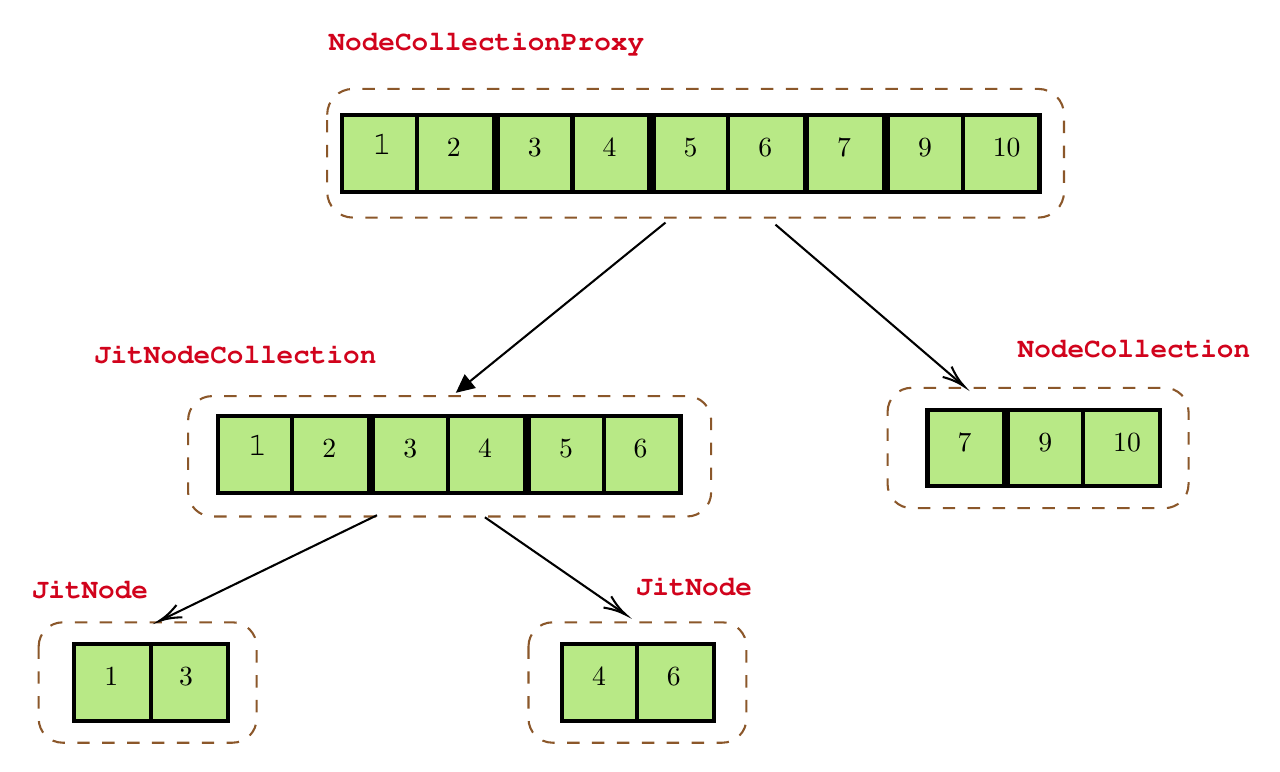
\begin{tikzpicture}[x=0.75pt,y=0.75pt,yscale=-1,xscale=1]
%uncomment if require: \path (0,426); %set diagram left start at 0, and has height of 426

%Shape: Square [id:dp8105017417201583] 
\draw  [color={rgb, 255:red, 0; green, 0; blue, 0 }  ,draw opacity=1 ][fill={rgb, 255:red, 184; green, 233; blue, 134 }  ,fill opacity=1 ][line width=1.5]  (164,92.5) -- (201,92.5) -- (201,129.5) -- (164,129.5) -- cycle ;
%Shape: Square [id:dp3649335086618113] 
\draw  [color={rgb, 255:red, 0; green, 0; blue, 0 }  ,draw opacity=1 ][fill={rgb, 255:red, 184; green, 233; blue, 134 }  ,fill opacity=1 ][line width=1.5]  (200,92.5) -- (237,92.5) -- (237,129.5) -- (200,129.5) -- cycle ;
%Shape: Square [id:dp6382262654140751] 
\draw  [color={rgb, 255:red, 0; green, 0; blue, 0 }  ,draw opacity=1 ][fill={rgb, 255:red, 184; green, 233; blue, 134 }  ,fill opacity=1 ][line width=1.5]  (239,92.5) -- (276,92.5) -- (276,129.5) -- (239,129.5) -- cycle ;
%Shape: Square [id:dp8010542992513336] 
\draw  [color={rgb, 255:red, 0; green, 0; blue, 0 }  ,draw opacity=1 ][fill={rgb, 255:red, 184; green, 233; blue, 134 }  ,fill opacity=1 ][line width=1.5]  (275,92.5) -- (312,92.5) -- (312,129.5) -- (275,129.5) -- cycle ;
%Shape: Square [id:dp31326160350937027] 
\draw  [color={rgb, 255:red, 0; green, 0; blue, 0 }  ,draw opacity=1 ][fill={rgb, 255:red, 184; green, 233; blue, 134 }  ,fill opacity=1 ][line width=1.5]  (314,92.5) -- (351,92.5) -- (351,129.5) -- (314,129.5) -- cycle ;
%Shape: Square [id:dp4264806381468127] 
\draw  [color={rgb, 255:red, 0; green, 0; blue, 0 }  ,draw opacity=1 ][fill={rgb, 255:red, 184; green, 233; blue, 134 }  ,fill opacity=1 ][line width=1.5]  (350,92.5) -- (387,92.5) -- (387,129.5) -- (350,129.5) -- cycle ;
%Shape: Square [id:dp0657777285734038] 
\draw  [color={rgb, 255:red, 0; green, 0; blue, 0 }  ,draw opacity=1 ][fill={rgb, 255:red, 184; green, 233; blue, 134 }  ,fill opacity=1 ][line width=1.5]  (388,92.5) -- (425,92.5) -- (425,129.5) -- (388,129.5) -- cycle ;
%Shape: Square [id:dp9110731509942587] 
\draw  [color={rgb, 255:red, 0; green, 0; blue, 0 }  ,draw opacity=1 ][fill={rgb, 255:red, 184; green, 233; blue, 134 }  ,fill opacity=1 ][line width=1.5]  (427,92.5) -- (464,92.5) -- (464,129.5) -- (427,129.5) -- cycle ;
%Shape: Square [id:dp8397495965826969] 
\draw  [color={rgb, 255:red, 0; green, 0; blue, 0 }  ,draw opacity=1 ][fill={rgb, 255:red, 184; green, 233; blue, 134 }  ,fill opacity=1 ][line width=1.5]  (463,92.5) -- (500,92.5) -- (500,129.5) -- (463,129.5) -- cycle ;
%Shape: Square [id:dp010231923951544264] 
\draw  [color={rgb, 255:red, 0; green, 0; blue, 0 }  ,draw opacity=1 ][fill={rgb, 255:red, 184; green, 233; blue, 134 }  ,fill opacity=1 ][line width=1.5]  (104,237.5) -- (141,237.5) -- (141,274.5) -- (104,274.5) -- cycle ;
%Shape: Square [id:dp40727955432554497] 
\draw  [color={rgb, 255:red, 0; green, 0; blue, 0 }  ,draw opacity=1 ][fill={rgb, 255:red, 184; green, 233; blue, 134 }  ,fill opacity=1 ][line width=1.5]  (140,237.5) -- (177,237.5) -- (177,274.5) -- (140,274.5) -- cycle ;
%Shape: Square [id:dp569596288283355] 
\draw  [color={rgb, 255:red, 0; green, 0; blue, 0 }  ,draw opacity=1 ][fill={rgb, 255:red, 184; green, 233; blue, 134 }  ,fill opacity=1 ][line width=1.5]  (179,237.5) -- (216,237.5) -- (216,274.5) -- (179,274.5) -- cycle ;
%Shape: Square [id:dp7015769826403364] 
\draw  [color={rgb, 255:red, 0; green, 0; blue, 0 }  ,draw opacity=1 ][fill={rgb, 255:red, 184; green, 233; blue, 134 }  ,fill opacity=1 ][line width=1.5]  (215,237.5) -- (252,237.5) -- (252,274.5) -- (215,274.5) -- cycle ;
%Shape: Square [id:dp6481677925435276] 
\draw  [color={rgb, 255:red, 0; green, 0; blue, 0 }  ,draw opacity=1 ][fill={rgb, 255:red, 184; green, 233; blue, 134 }  ,fill opacity=1 ][line width=1.5]  (254,237.5) -- (291,237.5) -- (291,274.5) -- (254,274.5) -- cycle ;
%Shape: Square [id:dp5988881062447686] 
\draw  [color={rgb, 255:red, 0; green, 0; blue, 0 }  ,draw opacity=1 ][fill={rgb, 255:red, 184; green, 233; blue, 134 }  ,fill opacity=1 ][line width=1.5]  (290,237.5) -- (327,237.5) -- (327,274.5) -- (290,274.5) -- cycle ;
%Shape: Square [id:dp3368376702520288] 
\draw  [color={rgb, 255:red, 0; green, 0; blue, 0 }  ,draw opacity=1 ][fill={rgb, 255:red, 184; green, 233; blue, 134 }  ,fill opacity=1 ][line width=1.5]  (446,234.5) -- (483,234.5) -- (483,271.5) -- (446,271.5) -- cycle ;
%Shape: Square [id:dp8793990825777143] 
\draw  [color={rgb, 255:red, 0; green, 0; blue, 0 }  ,draw opacity=1 ][fill={rgb, 255:red, 184; green, 233; blue, 134 }  ,fill opacity=1 ][line width=1.5]  (485,234.5) -- (522,234.5) -- (522,271.5) -- (485,271.5) -- cycle ;
%Shape: Square [id:dp5464263246257259] 
\draw  [color={rgb, 255:red, 0; green, 0; blue, 0 }  ,draw opacity=1 ][fill={rgb, 255:red, 184; green, 233; blue, 134 }  ,fill opacity=1 ][line width=1.5]  (521,234.5) -- (558,234.5) -- (558,271.5) -- (521,271.5) -- cycle ;
%Shape: Square [id:dp7930487300244025] 
\draw  [color={rgb, 255:red, 0; green, 0; blue, 0 }  ,draw opacity=1 ][fill={rgb, 255:red, 184; green, 233; blue, 134 }  ,fill opacity=1 ][line width=1.5]  (35,347.5) -- (72,347.5) -- (72,384.5) -- (35,384.5) -- cycle ;
%Shape: Square [id:dp5303377541943575] 
\draw  [color={rgb, 255:red, 0; green, 0; blue, 0 }  ,draw opacity=1 ][fill={rgb, 255:red, 184; green, 233; blue, 134 }  ,fill opacity=1 ][line width=1.5]  (72,347.5) -- (109,347.5) -- (109,384.5) -- (72,384.5) -- cycle ;
%Shape: Square [id:dp8774571362079038] 
\draw  [color={rgb, 255:red, 0; green, 0; blue, 0 }  ,draw opacity=1 ][fill={rgb, 255:red, 184; green, 233; blue, 134 }  ,fill opacity=1 ][line width=1.5]  (270,347.5) -- (307,347.5) -- (307,384.5) -- (270,384.5) -- cycle ;
%Shape: Square [id:dp5060305166010015] 
\draw  [color={rgb, 255:red, 0; green, 0; blue, 0 }  ,draw opacity=1 ][fill={rgb, 255:red, 184; green, 233; blue, 134 }  ,fill opacity=1 ][line width=1.5]  (306,347.5) -- (343,347.5) -- (343,384.5) -- (306,384.5) -- cycle ;
%Rounded Rect [id:dp7324795238782251] 
\draw  [color={rgb, 255:red, 139; green, 87; blue, 42 }  ,draw opacity=1 ][dash pattern={on 4.5pt off 4.5pt}] (156.8,92.4) .. controls (156.8,85.55) and (162.35,80) .. (169.2,80) -- (499.4,80) .. controls (506.25,80) and (511.8,85.55) .. (511.8,92.4) -- (511.8,129.6) .. controls (511.8,136.45) and (506.25,142) .. (499.4,142) -- (169.2,142) .. controls (162.35,142) and (156.8,136.45) .. (156.8,129.6) -- cycle ;
%Rounded Rect [id:dp8536055044343349] 
\draw  [color={rgb, 255:red, 139; green, 87; blue, 42 }  ,draw opacity=1 ][dash pattern={on 4.5pt off 4.5pt}] (89.8,239.6) .. controls (89.8,233.19) and (94.99,228) .. (101.4,228) -- (330.2,228) .. controls (336.61,228) and (341.8,233.19) .. (341.8,239.6) -- (341.8,274.4) .. controls (341.8,280.81) and (336.61,286) .. (330.2,286) -- (101.4,286) .. controls (94.99,286) and (89.8,280.81) .. (89.8,274.4) -- cycle ;
%Rounded Rect [id:dp7918544993903414] 
\draw  [color={rgb, 255:red, 139; green, 87; blue, 42 }  ,draw opacity=1 ][dash pattern={on 4.5pt off 4.5pt}] (426.8,235.6) .. controls (426.8,229.19) and (431.99,224) .. (438.4,224) -- (560.2,224) .. controls (566.61,224) and (571.8,229.19) .. (571.8,235.6) -- (571.8,270.4) .. controls (571.8,276.81) and (566.61,282) .. (560.2,282) -- (438.4,282) .. controls (431.99,282) and (426.8,276.81) .. (426.8,270.4) -- cycle ;
%Rounded Rect [id:dp667353387028452] 
\draw  [color={rgb, 255:red, 139; green, 87; blue, 42 }  ,draw opacity=1 ][dash pattern={on 4.5pt off 4.5pt}] (253.8,348.6) .. controls (253.8,342.19) and (258.99,337) .. (265.4,337) -- (347.2,337) .. controls (353.61,337) and (358.8,342.19) .. (358.8,348.6) -- (358.8,383.4) .. controls (358.8,389.81) and (353.61,395) .. (347.2,395) -- (265.4,395) .. controls (258.99,395) and (253.8,389.81) .. (253.8,383.4) -- cycle ;
%Rounded Rect [id:dp8903611832797551] 
\draw  [color={rgb, 255:red, 139; green, 87; blue, 42 }  ,draw opacity=1 ][dash pattern={on 4.5pt off 4.5pt}] (17.8,348.6) .. controls (17.8,342.19) and (22.99,337) .. (29.4,337) -- (111.2,337) .. controls (117.61,337) and (122.8,342.19) .. (122.8,348.6) -- (122.8,383.4) .. controls (122.8,389.81) and (117.61,395) .. (111.2,395) -- (29.4,395) .. controls (22.99,395) and (17.8,389.81) .. (17.8,383.4) -- cycle ;
%Straight Lines [id:da10260503749552963] 
\draw    (319.8,144.4) -- (221.13,224.51) ;
\draw [shift={(218.8,226.4)}, rotate = 320.93] [fill={rgb, 255:red, 0; green, 0; blue, 0 }  ][line width=0.08]  [draw opacity=0] (8.93,-4.29) -- (0,0) -- (8.93,4.29) -- cycle    ;
%Straight Lines [id:da9877013332650502] 
\draw    (372.8,145.4) -- (462.28,222.1) ;
\draw [shift={(463.8,223.4)}, rotate = 220.6] [color={rgb, 255:red, 0; green, 0; blue, 0 }  ][line width=0.75]    (10.93,-3.29) .. controls (6.95,-1.4) and (3.31,-0.3) .. (0,0) .. controls (3.31,0.3) and (6.95,1.4) .. (10.93,3.29)   ;
%Straight Lines [id:da062130966082328376] 
\draw    (180.8,285.4) -- (77.6,335.53) ;
\draw [shift={(75.8,336.4)}, rotate = 334.09] [color={rgb, 255:red, 0; green, 0; blue, 0 }  ][line width=0.75]    (10.93,-3.29) .. controls (6.95,-1.4) and (3.31,-0.3) .. (0,0) .. controls (3.31,0.3) and (6.95,1.4) .. (10.93,3.29)   ;
%Straight Lines [id:da44240203700368275] 
\draw    (232.8,286.4) -- (299.15,332.26) ;
\draw [shift={(300.8,333.4)}, rotate = 214.65] [color={rgb, 255:red, 0; green, 0; blue, 0 }  ][line width=0.75]    (10.93,-3.29) .. controls (6.95,-1.4) and (3.31,-0.3) .. (0,0) .. controls (3.31,0.3) and (6.95,1.4) .. (10.93,3.29)   ;

% Text Node
\draw (177,100.5) node [anchor=north west][inner sep=0.75pt]   [align=left] {{\fontfamily{pcr}\selectfont {\large 1}}};
% Text Node
\draw (213,102.5) node [anchor=north west][inner sep=0.75pt]   [align=left] {2};
% Text Node
\draw (252,102.5) node [anchor=north west][inner sep=0.75pt]   [align=left] {3};
% Text Node
\draw (288,102.5) node [anchor=north west][inner sep=0.75pt]   [align=left] {4};
% Text Node
\draw (327,102.5) node [anchor=north west][inner sep=0.75pt]   [align=left] {5};
% Text Node
\draw (363,102.5) node [anchor=north west][inner sep=0.75pt]   [align=left] {6};
% Text Node
\draw (401,102.5) node [anchor=north west][inner sep=0.75pt]   [align=left] {7};
% Text Node
\draw (440,102.5) node [anchor=north west][inner sep=0.75pt]   [align=left] {9};
% Text Node
\draw (476,102.5) node [anchor=north west][inner sep=0.75pt]   [align=left] {10};
% Text Node
\draw (117,245.5) node [anchor=north west][inner sep=0.75pt]   [align=left] {{\fontfamily{pcr}\selectfont {\large 1}}};
% Text Node
\draw (153,247.5) node [anchor=north west][inner sep=0.75pt]   [align=left] {2};
% Text Node
\draw (192,247.5) node [anchor=north west][inner sep=0.75pt]   [align=left] {3};
% Text Node
\draw (228,247.5) node [anchor=north west][inner sep=0.75pt]   [align=left] {4};
% Text Node
\draw (267,247.5) node [anchor=north west][inner sep=0.75pt]   [align=left] {5};
% Text Node
\draw (303,247.5) node [anchor=north west][inner sep=0.75pt]   [align=left] {6};
% Text Node
\draw (459,244.5) node [anchor=north west][inner sep=0.75pt]   [align=left] {7};
% Text Node
\draw (498,244.5) node [anchor=north west][inner sep=0.75pt]   [align=left] {9};
% Text Node
\draw (534,244.5) node [anchor=north west][inner sep=0.75pt]   [align=left] {10};
% Text Node
\draw (48,357.5) node [anchor=north west][inner sep=0.75pt]   [align=left] {1};
% Text Node
\draw (84,357.5) node [anchor=north west][inner sep=0.75pt]   [align=left] {3};
% Text Node
\draw (283,357.5) node [anchor=north west][inner sep=0.75pt]   [align=left] {4};
% Text Node
\draw (319,357.5) node [anchor=north west][inner sep=0.75pt]   [align=left] {6};
% Text Node
\draw (43,202) node [anchor=north west][inner sep=0.75pt]   [align=left] {{\fontfamily{pcr}\selectfont \textcolor[rgb]{0.82,0.01,0.11}{\textbf{JitNodeCollection}}}};
% Text Node
\draw (488,199) node [anchor=north west][inner sep=0.75pt]   [align=left] {{\fontfamily{pcr}\selectfont \textcolor[rgb]{0.82,0.01,0.11}{\textbf{NodeCollection}}}};
% Text Node
\draw (13,315) node [anchor=north west][inner sep=0.75pt]   [align=left] {{\fontfamily{pcr}\selectfont \textcolor[rgb]{0.82,0.01,0.11}{\textbf{JitNode}}}};
% Text Node
\draw (304,314) node [anchor=north west][inner sep=0.75pt]   [align=left] {{\fontfamily{pcr}\selectfont \textcolor[rgb]{0.82,0.01,0.11}{\textbf{JitNode}}}};
% Text Node
\draw (156,51) node [anchor=north west][inner sep=0.75pt]   [align=left] {{\fontfamily{pcr}\selectfont \textcolor[rgb]{0.82,0.01,0.11}{\textbf{NodeCollectionProxy}}}};


\end{tikzpicture}

    \caption{From list to \emph{tree-like} structure: The initial \texttt{NodeCollectionProxy} has 9 items. The first 6 items are from the \texttt{JitNodeCollection} and the last 3 are from the \texttt{nest.NodeCollection}. The six items  in \texttt{JitNodeCollection} are from two different models, and these instances of the models are represented by the \texttt{JitNode}. The first \texttt{JitNode} spans a contiguous space of \emph{ids} between 1 and 3. The second \texttt{JitNode} spans another contiguous space between 4 and 6.}
    \label{fig:list_to_tree}
\end{figure}


Due to the structure that the \texttt{NodeCollectionProxy} is not really a list of element, but instead a \emph{tree-like} structure as depicted in \autoref{fig:list_to_tree}. Retrieving an element from the \texttt{NodeCollection} at position $i$ is not very a straightforward task. Since the root has only two children nodes, we check if $i$ is less than the size of the \texttt{JitNodeCollection}, otherwise we choose the \texttt{NodeCollection}. If $i$ ends up in the range of the \texttt{JitNodeCollection}, then we check if $i$ belongs to one of the \texttt{JitNode} blocks. Assuming we have $n$ \texttt{JitNode} blocks and each block points to $k_j$ instances of any arbitrary model $m$ for $j \in [1, n]$. A \texttt{JitNode} block  $b_l$ is selected with $ l \in [1, n)$ if
$\sum_{j=1}^{l-1} len(b_j) \leq i < \sum_{j=1}^{l-1} len(b_j) + len(b_l)$. Once the block $b$ is found, we can convert the \texttt{global id} $i$ to the \emph{local id} with respect to the found block $b_l$. Thus, the \emph{local id} is computed as  $ local_{id} = i -\sum_{j=1}^{l-1} len(b_j)$. Since the \texttt{JitNode} is \emph{indexable}, we can simply get a new \texttt{JitNode} having in the \texttt{first} attribute the $local_{id}$ as value and for the \texttt{last} attribute the value $local_{id} + 1$ and finally the \texttt{model\_name} will be set to $m$. The result then for querying the \texttt{NodeCollectionProxy} to return the element at the position $i$ will be a new \texttt{NodeCollectionProxy} with the size of one,  and it contains only a \texttt{JitNodeCollection}. The \texttt{JitNodeCollection} instance will have a single \texttt{JitNode} object pointing to one element. To illustrate an example, let's take the \texttt{NodeCollectionProxy} in \autoref{fig:list_to_tree} with ten elements and let $i = 5$. The \texttt{JitNodeCollection} has six elements and the \texttt{NodeCollection} has only four, and therefore $i=5$ ends up in the \texttt{JitNodeCollection} child. For the first \texttt{JitNode} in the \texttt{JitNodeCollection} we have three items, in the second one we have two elements, and therefore we have $l \in \{1, 2\}$. For $l=1$, we have $0 \leq i = 5$ and $5 \not < 0 + len(b_l) = 0 + len(b_1) = 0 + 3 = 3$. For $l=2$, we $0 + len(b_1) = 0 + 3 \leq 5$ and $5 < len(b_1) + len(b_2) = 3 + 3 = 6.$ In that case, it seems that $l=2$ satisfies the required condition, and therefore $i=5$ belongs to the second \texttt{JitNode} block. The result then will be a \texttt{NodeCollectionProxy} with only a \texttt{JitNodeCollection} child, which has a single \texttt{JitNode = <first= 5 - 4, last=6, name=$m$>}, with four is the index where the second \texttt{JitNode} starts and $m$ is the name of the model.


\emph{Slicing} a \texttt{NodeCollectionProxy} is basically similar to indexing, with the only difference that we have a sequence of items $(a_1, \dots, a_k)$, with $k$ the size of the sequence. The problem with \emph{slicing} is that the items are not necessary the direct successors of each other. In other words, it may be possible that $a_{i+1} =a_i + l$, for $l > 1$, and $a_i$ and $a_{i+1}$ might point to different \texttt{JitNode}s. In order to solve that problem, we start by mapping each $a_i$ to the corresponding \texttt{JitNode} block, then we group all items together that share the same block. For each group, we convert the \emph{global ids} $a_i$ to the relative \emph{local ids} in each \texttt{JitNode} block. By doing so, we should have the following mapping: $(a_1, a_2, \dots, a_k) \mapsto (P_1, \dots P_l)$, with $\lvert\bigcup_{i=1}^{l} P_{i}\rvert =n$. $P_i$ is the partition of the
items containing the \emph{local ids} of the original sequence. For each partition $P_i$, we aggregate the elements inside them in a way that each group is a contiguous group of \emph{ids}. Each of these groups then constructs a new \texttt{JitNode} and all the new \texttt{JitNode}s will be packed in a new \texttt{JitNodeCollection}.


Basically, for \emph{indexing} and \emph{slicing}, we iterate over the \emph{tree-like} structure twice. In the first iteration, we examine the tree from the top to the bottom by mapping the \emph{global ids} to \emph{local ids} and retrieve the correct \texttt{JitNode} instances. The second iteration, we traverse the tree from the bottom to top by merging and aggregating the results together until constructing the final \texttt{NodeCollectionProxy}. Getting or setting the value of certain \emph{keys} in the \texttt{NodeCollectionProxy} undergoes the same logic. By requesting the value of some \emph{keys}, the \texttt{NodeCollectionProxy} asks both the \texttt{NodeCollection} and the \texttt{JitNodeCollection} to retrieve the value of given keys. In return, the \texttt{JitNodeCollection} does also the same by asking each of the \texttt{JitNode} blocks. The returned value will be either the correct value that is stored in instances of the model or a \texttt{NoneType} object, indicating that the model does not have the requested \emph{key} as an attribute. Again, the result from each level will be aggregated and delivered to a higher level in the tree until we reach the root (i.e., the \texttt{NodeCollectionProxy}). The \emph{set} function in the \texttt{NodeCollectionProxy} has the exact behavior as the \emph{get} function, with the single different that the new values will be split among the children in a way that  each child gets a sub-dictionary containing only its proper \emph{keys}.

\subsection{The JitModelParser}

Generating the code for the \emph{lightweight} version of the model undergoes practically the same logic as generating the code for the whole library.  The \texttt{JitModelParse} is the component responsible for creating the \emph{lightweight} version. The component takes as an input the \texttt{ASTNeuron} and returns as an output an executable \texttt{C++} code. Mainly, the \texttt{C++} code contains the declared \emph{State} block and the \emph{Parameter} block, including the \emph{constructor} that is responsible for initializing the attributes in those blocks. Additionally, some of these attributes might  be assigned a random value drawn from a well-supported distribution in the \emph{NestKernel}. The problem here is that the random number generator is purely coming from the \texttt{NestKernel} library, and we do not really want to include anything related to the \emph{NestKernel} at this point. Furthermore, it is very important to preserve the order in which the random numbers are drawn to ensure the \emph{reproducibility} of the simulation results.

Luckily, to tackle this problem, the \texttt{JitModelParser} extracts the \emph{symbols} referring to the random number generator in the \texttt{C++} generated code for the \emph{lightweight} version from the \emph{constructor} and replaces them with a variable. The declaration of this variable will be inserted in the \emph{constructor}. Thus, if we have $n$ statements in the \emph{constructor} that use a random number generator in their expression, then we replace the occurrences of each of these generators with a new variable $r_i$, for $i \in [1, n]$ and extend the \emph{constructor} with $n$ new parameters in the form of $\texttt{double } r_i$. The \texttt{JitModelParse} compiles the \emph{lightweight} version and makes the new class available in the Python interface with the help of the \emph{CPPYY} module \citep{cppyy}. The \texttt{JitModelParse} is also responsible for calling the extended constructor, and provides the value of the new added parameters. It simply calls the \emph{PyNEST} functions responsible for generating the random numbers and passing them to the \emph{lightweight} version class constructor to initialize its attributes in the \emph{State} and \emph{Parameters} blocks.

Unfortunately, the \texttt{lightweight} version requires having a duplicate space for the model's attributes. Those coming from the \texttt{lightweight} model  and the others after completing building the library and creating the real instance of the model. Also, drawing the random numbers is done on a single computing node, and it might influence the results and performance if more computing nodes are used. To tackle this problem and partially solve it, we decided to make the \emph{model} more modular that can be decomposed into independent interchangeable subcomponents. More to the \emph{modularity} will be discussed in the next chapter.

\section{PyNEST: The Connect Function}

Previously, all used neuron-synapse combinations involving synapse models with a dependency on post-synaptic variables, such as spike-timing dependent plasticity (STDP), had to be provided manually to the code generator before running the simulation.  This dependency is now hidden in the \texttt{ConnectWrapper} that extends the functionality of the \texttt{nest.Connect} function and depending on the synaptic connection, the code generation process might be triggered  for the second time after being called in the \texttt{nest.Create}, but this time with different  configurations that allow the code co-generation of the neuron model and its synaptic element.

\subsection{The ConnectWrapper}

The \texttt{ConnectWrapper} with its three core functions (i.e., \texttt{before-main-after}) intercepts the calls to the \texttt{nest.Connect} function, ensuring the correct use of models during building of the network. The \texttt{before} functions have mainly the same signature as the \texttt{nest.Connect}. It takes a source as the presynaptic part of the connection, a target as the postsynaptic element. Additionally, the function takes two dictionaries, one for specifying the connection specification such as the connectivity rule between the source and the target. The second dictionary is for specifying the synapse model and its properties. The task of the \texttt{before} function in the context of building the connections in the network is to make sure that both source and target are the real instances of the models and the \texttt{NodeCollectionProxy} contains only a \texttt{NodeCollection} whereas the \texttt{JitNodeCollection} is empty. 

The \texttt{before} function starts by checking if either the target (postsynaptic element) is a \texttt{NodeCollectionProxy} containing a \texttt{JitNodeCollection} child and the synapse model type is an external model. If both requirements are satisfied and, depending on the situation, if both the postsynaptic neuron and the synapse are already existing in a library or coming from a \emph{nestml} files. The \texttt{before} function delegate the work to the \texttt{ConnectHelper} that takes care of converting the postsynaptic nodes residing in the \texttt{JitNodeCollection} to the real instances. Next, we check if the source and target are contained inside a \texttt{JitNodeCollection}, which means they are at least two \emph{threads} running and building the code for the source and target neurons models. We then explicitly wait for these two threads, and when they finish without any failure, we install the two libraries built by the threads and convert the \texttt{JitNodeCollection} objects from the source and target to the \texttt{NodeCollection} objects. Depending on the order of calling the \texttt{nest.Connect}, we might need to delete certain connections and replace them with others. 

From the \emph{JIT} perspective upon calling the \texttt{nest.Create} function, we do not really know what will happen to the model and which connections it will have, and it is only really known when calling the \texttt{nest.Connect} function. Thus having a \texttt{nest.Connect} function that connects the source and the target with
an external synapse model will require deleting connections and replacing them with others. The reason behind the deletion and replacing of the edges is because the target neuron model will be assigned a new name from the code generation pipeline and the actual target model will not be valid anymore. Of course, if we call this particular  \texttt{nest.Connect} function with the external synapse type as the first function involving that postsynaptic neuron, then no deletion or replacing will be required, and the new neuron model will be directly available to all subsequent calls to the \texttt{nest.Connect} function. As the final step, the \texttt{before} function returns the converted \texttt{JitNodeCollection} to \texttt{NodeCollection} together with the other parameters as input parameters to the \texttt{main} function in the \texttt{ConnectWrapper}. Both the \texttt{main} and \texttt{after} functions are the default implementation from the \texttt{Wrapper}, and therefore the \texttt{main} function just calls the real \texttt{nest.Connect} function and the \texttt{after} does nothing.


\subsection{The ConnectHelper}


The \texttt{ConnectHelper} is mainly responsible for checking the state of the threads that are involved in building the library of the models specified in the connect call. It installs the libraries and converts the \texttt{JitNodeCollection} to the \texttt{NodeCollection}. It handles the use case when the co-code generation pipeline must be triggered again and takes care of deleting and replacing the connections of the involved models.


The \texttt{wait\_for\_threads} method takes as parameters a list of \emph{strings} containing the name of threads that we must wait for. The threads names are basically the names of the model they are building the library for. The function waits for the specified threads and inspects their states once they are done building the library and, depending on the state, we either continue the execution of the \texttt{ConnectWrapper} or throw a failure message and stop the execution of the simulation script. Finally, the function removes the terminated threads from the list of running threads. The list will be either further processed by another connect call or the \texttt{nest.Simulate} function.

Next, we have the \texttt{install\_modules} method, and it takes the same parameters as the  \texttt{wait\_for\_threads} function. The function is mainly responsible for installing the libraries, calling the \texttt{nest.SetDefaults} for models that have their default values changed under the provided list of models, coping models by calling \texttt{nest.CopyModels} in case if one of the given models must be copied with different initial values.

One of the important functions in the \texttt{ConnecetHelper} is handling the conversion of the postsynapse neuron when an external synapse model is involved. The \texttt{convert\_post\_neuron} takes as parameters a \texttt{NodeCollectionProxy} and the name of the synapse model. Depending on the involved elements, we distinguish nine distinct use cases when applying the conversion. Each of the neurons and synapse can be either from a \emph{nestml} file, an \emph{external library} or already are \emph{built\_in} models. Therefore, we can build a pair where the first position indicates the source of the neuron and the second is for the source of the synapse model. The first pair is \emph{(nestml, nestml}), which means that both models are only found in the \emph{nestml} format. Therefore, we have the  \emph{handle\_nestml\_nestml} function that is responsible for starting the code generation phase to generate the code for the new model that exclusively supports the synapse model. The function does not parse again both models, but it retrieves them from the \texttt{JitModels} as both should have been already parsed and validated. The function only triggers the transformation phase, as some attributes from the synapse will be transferred to the neuron model. Once the code generation is completed and the library is installed, the function creates the real instance of the model and returns the new \texttt{NodeCollection} objects to be used further in the main function in the \texttt{ConnectWrapper}. The second pair is then the \emph{(external, nestml}), which when the neuron model is already exists in some external library and the synapse model is only in a \emph{nestml} format. The function in that case tries to find the \emph{nestml} version of the model, and if it is found, it will then execute the same logic as in the previous pair case. If the \emph{nestml} of the model is not found, then we just throw an error and stop the execution, as it is not possible to bind the synapse with the model without having extra information how to generate the code of the \emph{neuron-synapse} model. 

The next pair is the \emph{(built\_in, nestml)} case, where the neuron model is a \emph{built\_in} model and the synapse from a \emph{nestml} file. This case requires a prior conditions to be satisfied in order to continue the execution of the \texttt{nest.Connect} function. In general, if the target model name is \emph{x} and the synapse name is \emph{y}, and we want to connect with the source and target with the \emph{y}, then the name type of the target model must be an instance of the \emph{x\_\_with\_y} and the synapse also will be assigned a new name as \emph{y\_\_with\_x}. In general, the synapse and the neuron code are complied and built in the same library, so that if \emph{y\_\_with\_x} is installed then also is the \emph{x\_\_with\_y} and vice-versa. In this particular case, we search if the  synapse \emph{y\_\_with\_x} can be found in any of the existing libraries and install it, which should then also register the \emph{x\_\_with\_y} neuron model, and then we can continue creating the \texttt{NodeCollection} object.


Finally, we have the \emph{(built\_in, built\_n)} that both neuron and synapse are already available in the \emph{NestKernel}. As in the previous case, it is required that both the \emph{x\_\_with\_y} and the \emph{y\_\_with\_x} are registered, or we will just then stop the execution of the simulation script and throw the error that we can not find the models. In all the other remaining cases, we just do nothing and let the \texttt{nest.Connect} handle them.


At the last function in the \texttt{ConnectWrapper}, we have the \texttt{convet\_to\_node\_collection} that converts an instance of the \texttt{JitNodeCollection} to a \texttt{NodeCollection} and updates the new created instance by the assigned values to the model. It is important to know the difference between the \texttt{convet\_to\_node\_collection} and the \texttt{convet\_post\_neuron}, as for the second function is only called to convert the target \texttt{NodeCollectionProxy} if there is an external synapse model involved and the first function just converts any \texttt{JitNodeCollection} without any prior requirements apart from the model's library being already installed in the \emph{NestKernel}.
   
\section{PyNEST: The Simulation Function}
   
The \texttt{nest.Simulate} method is intercepted by the \texttt{SimulateWrapper} that exactly does the same as the \texttt{ConnectWrapper}, but instead of having only models extracted from the source and target in the connect function, we apply the functions for all models. In other words, all the threads until running the \emph{simulate} function must be awaited for, and their states will be examined for any failure and subsequently, all libraries built by the threads will be installed and then all \texttt{JitNodeCollection} instances existing in the simulation script will be converted to a \texttt{NodeCollection} objects, even those coming from \emph{slicing} and \emph{indexing}. Like any custom implemented \texttt{Wrapper}, the \texttt{SimulateWrapper} uses the \texttt{SimulateHelper} that implements the above-mentioned functionalities.






\section{Usage}

Here we reach in the end of this chapter by showing the new changes that must be applied at the simulation level to adjusted when using the \emph{JIT} module.
For the purpose of the following demonstrations, we will use the \emph{STDP windows tutorial} from the official \emph{NESTML} website in order to show the new adjustments made by \emph{JIT} tool to facilitate the work for the simulation script.

 

The first changes that are affected by using  the \emph{JIT} approach happens at the \emph{import} level in the simulation script. As depicted in the \autoref{lst:imports_without_jit} and \autoref{lst:imports_with_jit}, we see that only the first three lines involving both the \emph{PyNEST} and the \emph{PyNESTML} modules are completely deleted and replaced with a single import call to the \texttt{nest} module from the \emph{JIT} the module. Apart from these changes, the rest of the import lines stay unchanged. 

\begin{figure}[ht!]
\centering
\begin{lstlisting}[language=Python, label=lst:imports_without_jit, caption={The Simulation script imports without JIT}]
import nest
from pynestml.frontend.pynestml_frontend import generate_nest_target
NEST_SIMULATOR_INSTALL_LOCATION = nest.ll_api.sli_func("statusdict/prefix ::")

%matplotlib inline
import matplotlib as mpl
mpl.rcParams['axes.formatter.useoffset'] = False
import matplotlib.pyplot as plt
import numpy as np
import os
import re

\end{lstlisting}
%\caption{The Simulation script imports without \emph{JIT}}
%\label{fig:imports_without_jit}
\end{figure}

\begin{figure}[ht!]
\centering
\begin{lstlisting}[language=Python, label=lst:imports_with_jit, caption={The Simulation script imports with JIT}]
from jit import nest

%matplotlib inline
import matplotlib as mpl
mpl.rcParams['axes.formatter.useoffset'] = False
import matplotlib.pyplot as plt
import numpy as np
import os
import re
\end{lstlisting}
\caption{The Simulation script imports \emph{JIT}}
%\label{fig:imports_with_jit}
\end{figure}

Secondly, in the \emph{NESTML} tutorial, we have the \texttt{generate\_code\_for} in \autoref{lst:generating_code} that takes as parameter the synapse model name. The function retrieves the \emph{nestml} file for the given synapse and also the \emph{nestml} file for the \texttt{iaf\_psc\_delta} neuron model and then triggers the co-code generation for both models together providing the \texttt{post\_ports} that required for connecting the postsynaptic neuron together with the synapse. Finally, once the code generation pipeline finishes, it installs the new library, which makes the specified model available for use in the simulation script and returns the new expected name of the neuron and synapse that both have the \emph{\_\_with\_} infix. Luckily, using the \emph{JIT} tool, we can simply get rid of this huge function and let it completely take care of the models, and their new names. Even the \texttt{nest.Install} function on the line 41 will also be deleted, and only the \emph{JIT} is responsible for calling it.



Finlay, we reach the part where we have to create the nodes and connect them to build the network. Both the figures \autoref{lst:build_network_with_jit} and \autoref{lst:build_network_without_jit} share the exact the code, apart from a slight difference in the line 44 when calling the \texttt{nest.Connect} function. In the figure \autoref{lst:build_network_with_jit} we add an extra key in the \texttt{syn\_spec} indicating the \emph{post connection ports} between the synapse and the post-neuron. The new key then will be removed from the \texttt{syn\_spec} dictionary and only be used in the code generation pipeline as one of the custom configurations in the \emph{codegen\_opt} in \emph{PyNESTML} module. The rest of the dictionary is then forwarded to \texttt{ConnectWrapper} to initiate the correct call to the \texttt{nest.Connect} function.

In short, the \emph{JIT} design and implementation does not affect the workflow of the simulation script and only slight changes are required to be adjusted without a huge intervention from the user.

\section{Summary}

We started by understanding the working environment between the three main components in this project. The \emph{PyNESTML} module for generating the code of the external modules, \emph{PyNEST} the high level \emph{API} for creating the nodes of the network and connecting them, and finally, we  have \emph{NestKernel} as the core of the simulation that manages its execution and delivers results back to the \emph{PyNEST} module. After that, we understood the basic workflow between them, we derived the necessary requirements that should be satisfied by the \emph{JIT} design. Finally, we explained the most important components involved in the \emph{JIT} module and how each piece is necessary for intercepting the calls from the \emph{PyNEST} and seamlessly modifying their execution paths, either by adding new functionalities or totally skipping the function and executing something different.


Two major drawbacks in the implemented solution, that the assigned values to the attributes of the model will be stored twice in the memory. The first values come from storing the \emph{lightweight} version of the model, and the second values come after creating the real instances of the model in the \texttt{nest.Connect} and \texttt{nest.Simulate} calls. The second drawback is triggering the code generation pipeline twice when trying to connect a post-neuron with an external synapse type. To tackle these two problems, we decided to make the neuron models more flexible and modular that can be assembled in the runtime, instead of writing the whole code and compiling it into one single library. But in order to make the \texttt{NestKernel} support modularity and make it utilize its potential, we need to implement a new data structure for the models that should make the transition between the normal models and the modular ones more flexible. In the next chapter, we should introduce this new data structure and discuss its strong connection with the modularity.

\begin{figure}[ht!]
%\caption{The code-generation phase}
\thisfloatpagestyle{empty} 
\begin{lstlisting}[language=Python, label=lst:generating_code, caption={The code-generation phase}]
n_modules_generated = 0
def generate_code_for(nestml_synapse_model: str):
    """Generate code for a given synapse model, passed as a string, in combination with
    the iaf_psc_delta model.

    NEST cannot yet reload modules. Workaround using counter to generate unique names."""
    global n_modules_generated

    # append digit to the neuron model name and neuron model filename
    with open("models/neurons/iaf_psc_delta.nestml", "r") as nestml_model_file_orig:
        nestml_neuron_model = nestml_model_file_orig.read()
        nestml_neuron_model = re.sub("neuron\ [^:\s]*:",
                                     "neuron iaf_psc_delta" + str(n_modules_generated) + ":", nestml_neuron_model)
        with open("models/neurons/iaf_psc_delta" + str(n_modules_generated) + ".nestml", "w") as nestml_model_file_mod:
            print(nestml_neuron_model, file=nestml_model_file_mod)

    # append digit to the synapse model name and synapse model filename
    nestml_synapse_model_name = re.findall("synapse\ [^:\s]*:", nestml_synapse_model)[0][8:-1]
    nestml_synapse_model = re.sub("synapse\ [^:\s]*:",
                                  "synapse " + nestml_synapse_model_name + str(n_modules_generated) + ":", nestml_synapse_model)
    with open("models/synapses/" + nestml_synapse_model_name + str(n_modules_generated) + ".nestml", "w") as nestml_model_file:
        print(nestml_synapse_model, file=nestml_model_file)

    # generate the code for neuron and synapse (co-generated)
    module_name = "nestml_" + str(n_modules_generated) + "_module"
    generate_nest_target(input_path=["models/neurons/iaf_psc_delta" + str(n_modules_generated) + ".nestml",
                                     "models/synapses/" + nestml_synapse_model_name + str(n_modules_generated) + ".nestml"],
                         target_path="/tmp/nestml_module",
                         logging_level="ERROR",
                         module_name=module_name,
                         suffix="_nestml",
                         codegen_opts={"nest_path": NEST_SIMULATOR_INSTALL_LOCATION,
                                       "neuron_parent_class": "StructuralPlasticityNode",
                                       "neuron_parent_class_include": "structural_plasticity_node.h",
                                       "neuron_synapse_pairs": [{"neuron": "iaf_psc_delta" + str(n_modules_generated),
                                                                   "synapse": nestml_synapse_model_name + str(n_modules_generated),
                                                                   "post_ports": ["post_spikes"]}]})

    # load module into NEST
    nest.ResetKernel()
    nest.Install(module_name)

    mangled_neuron_name = "iaf_psc_delta" + str(n_modules_generated) + "_nestml__with_" + nestml_synapse_model_name + str(n_modules_generated) + "_nestml"
    mangled_synapse_name = nestml_synapse_model_name + str(n_modules_generated) + "_nestml__with_iaf_psc_delta" + str(n_modules_generated) + "_nestml"

    n_modules_generated += 1

    return mangled_neuron_name, mangled_synapse_name
\end{lstlisting}

%\label{fig:generating_code}
\end{figure}

\clearpage


\begin{figure}[ht!]
\centering
%\caption{}
\begin{lstlisting}[language=Python, label=lst:build_network_without_jit, caption={Creating the network without \emph{JIT}}]
def run_network(pre_spike_time, post_spike_time,
                          neuron_model_name,
                          synapse_model_name,
                          resolution=1., # [ms]
                          delay=1., # [ms]
                          lmbda=1E-6,
                          sim_time=None,  # if None, computed from pre and post spike times
                          synapse_parameters=None,  # optional dictionary passed to the synapse
                          fname_snip=""):

    nest.set_verbosity("M_WARNING")
    #nest.set_verbosity("M_ALL")

    nest.ResetKernel()
    nest.SetKernelStatus({'resolution': resolution})

    wr = nest.Create('weight_recorder')
    nest.CopyModel(synapse_model_name, "stdp_nestml_rec",
                {"weight_recorder": wr[0],
                 "w": 1.,
                 "delay": delay,
                 "d": delay,
                 "receptor_type": 0,
                 "mu_minus": 0.,
                 "mu_plus": 0.})

    # create spike_generators with these times
    pre_sg = nest.Create("spike_generator",
                         params={"spike_times": [pre_spike_time, sim_time - 10.]})
    post_sg = nest.Create("spike_generator",
                          params={"spike_times": [post_spike_time],
                                  'allow_offgrid_times': True})

    # create parrot neurons and connect spike_generators
    pre_neuron = nest.Create("parrot_neuron")
    post_neuron = nest.Create(neuron_model_name)

    spikedet_pre = nest.Create("spike_recorder")
    spikedet_post = nest.Create("spike_recorder")
    #mm = nest.Create("multimeter", params={"record_from" : ["V_m"]})

    nest.Connect(pre_sg, pre_neuron, "one_to_one", syn_spec={"delay": 1.})
    nest.Connect(post_sg, post_neuron, "one_to_one", syn_spec={"delay": 1., "weight": 9999.})
    nest.Connect(pre_neuron, post_neuron, "all_to_all", syn_spec={'synapse_model': 'stdp_nestml_rec'})
    #nest.Connect(mm, post_neuron)

    nest.Connect(pre_neuron, spikedet_pre)
    nest.Connect(post_neuron, spikedet_post)
    
    nest.Simulate(sim_time)
    
    # rest is retrieving results from spikes
    ...

\end{lstlisting}
%\label{fig:build_network_without_jit}
\end{figure}

\clearpage

\begin{figure}[ht!]
\centering
%\caption{Creating the network with \emph{JIT}}

\begin{lstlisting}[language=Python, label=lst:build_network_with_jit, caption={Creating the network with JIT}]
def run_network(pre_spike_time, post_spike_time,
                          neuron_model_name,
                          synapse_model_name,
                          resolution=1., # [ms]
                          delay=1., # [ms]
                          lmbda=1E-6,
                          sim_time=None,  # if None, computed from pre and post spike times
                          synapse_parameters=None,  # optional dictionary passed to the synapse
                          fname_snip=""):

    nest.set_verbosity("M_WARNING")
    #nest.set_verbosity("M_ALL")

    nest.ResetKernel()
    nest.SetKernelStatus({'resolution': resolution})

    wr = nest.Create('weight_recorder')
    nest.CopyModel(synapse_model_name, "stdp_nestml_rec",
                {"weight_recorder": wr[0],
                 "w": 1.,
                 "delay": delay,
                 "d": delay,
                 "receptor_type": 0,
                 "mu_minus": 0.,
                 "mu_plus": 0.})

    # create spike_generators with these times
    pre_sg = nest.Create("spike_generator",
                         params={"spike_times": [pre_spike_time, sim_time - 10.]})
    post_sg = nest.Create("spike_generator",
                          params={"spike_times": [post_spike_time],
                                  'allow_offgrid_times': True})

    # create parrot neurons and connect spike_generators
    pre_neuron = nest.Create("parrot_neuron")
    post_neuron = nest.Create(neuron_model_name)

    spikedet_pre = nest.Create("spike_recorder")
    spikedet_post = nest.Create("spike_recorder")
    #mm = nest.Create("multimeter", params={"record_from" : ["V_m"]})

    nest.Connect(pre_sg, pre_neuron, "one_to_one", syn_spec={"delay": 1.})
    nest.Connect(post_sg, post_neuron, "one_to_one", syn_spec={"delay": 1., "weight": 9999.})
    nest.Connect(pre_neuron, post_neuron, "all_to_all", syn_spec={'synapse_model': 'stdp_nestml_rec', "post_ports": ["post_spikes"]})
    #nest.Connect(mm, post_neuron)

    nest.Connect(pre_neuron, spikedet_pre)
    nest.Connect(post_neuron, spikedet_post)
    
    nest.Simulate(sim_time)
    
    # rest is retrieving results from spikes
    ...

\end{lstlisting}
%\label{fig:build_network_with_jit}
\end{figure}

\cleardoublepage
